\documentclass[a4paper, 11pt, english]{report}
 
\usepackage[a4paper,
            width=34em,
            headheight=13.6pt,
            top=10em,
            bottom=12em]{geometry}     % for slightly wider margins. Save trees
\usepackage[svgnames,hyperref]{xcolor} % To define colors
\usepackage[utf8]{inputenc}            % UTF-8 and symbol support
\usepackage[english]{babel}            % for proper word breaking at line ends
\usepackage[final,
            tracking,
            babel,
            kerning,
            spacing]{microtype} % to fix words clipping outside of bounds. A must have
\SetTracking{encoding=*, shape=sc}{50} % microtype: fixes weird width in small caps
%\usepackage[all]{nowidow}
\usepackage[autostyle=true]{csquotes}  % because biblatex needs it
\setlength {\marginparwidth }{3cm}     % for better margins for the todo notes
\usepackage[backgroundcolor=BlanchedAlmond, 
            linecolor=BurlyWood, 
            obeyFinal]{todonotes}      % notes for during development
\usepackage{parskip}                   % New paragraphs are 1 line apart and not indented.
\usepackage{enumitem}                  % for better enumerate, itemize, and description.
%\usepackage[normalem]{ulem}           % To strikethrough text
\GetGinDriver
\usepackage[\GinDriver,
            pdfusetitle,
            pdfsubject={A Master Thesis in Computer Science at the Radboud University},
            pdfkeywords={Windows, process migration, checkpointing, malware analysis},
            colorlinks=true,
            citecolor=DeepPink,
            linkcolor=Navy,
            urlcolor=Navy]{hyperref}   % for urls and referations
\usepackage[backend=biber,
            natbib=true,
            dashed=false,
            style=ieee]{biblatex}      % for \citeauthor and \cite
\addbibresource{reference.bib}

\renewcommand{\arraystretch}{1.3}      % for more space between table rows

\usepackage{fancyhdr}                  % for the header
\pagestyle{fancy}
\fancyhead{}
\fancyhead[LO,RE]{\textsl{\leftmark}}

\usepackage{listings}                  % for code blocks

\lstdefinestyle{mystyle}{
	backgroundcolor=\color{GhostWhite},
	commentstyle={\color{ForestGreen}},
	keywordstyle=\color{DodgerBlue},
	numberstyle=\color{DimGrey},
	stringstyle=\color{IndianRed},
	basicstyle=\ttfamily\scriptsize,
	breakatwhitespace=false,
	breaklines=true,
	captionpos=b,
	keepspaces=true,
	numbers=left,
	numbersep=5pt,
%	numberstyle=\emptyaccsupp,
	showspaces=false,
	showstringspaces=false,
	showtabs=false,
	tabsize=4,
}
\lstset{
	language={[Visual]C++},
	style=mystyle,
}



\def\thesistitle{Towards process migration in Windows 10 }
\def\thesissubtitle{Moving a running process from one machine to another}
\def\thesisauthorfirst{Wietze D.}
\def\thesisauthorsecond{Mulder}
\def\thesissupervisorfirst{dr. ir. Erik}
\def\thesissupervisorsecond{Poll}
\def\thesissecondreaderfirst{drs. Pol}
\def\thesissecondreadersecond{Van Aubel}
\def\thesisdate{July 12, 2023}

%% FOR PDF METADATA
\title{\thesistitle}
\author{\thesisauthorfirst\space\thesisauthorsecond}
\date{\thesisdate}

\begin{document}

\makeatletter

% To get the cool roman page numbering before the introduction
\newcommand\frontmatter{%
    \cleardoublepage
  %\@mainmatterfalse
  \pagenumbering{roman}}

\newcommand\mainmatter{%
    \cleardoublepage
 % \@mainmattertrue
  \pagenumbering{arabic}}

%\frontmatter

% These commands have to be after \begin{document} (idk why)
\renewcommand{\chapterautorefname      }{Chapter} % default: chapter
\renewcommand{\sectionautorefname      }{Section} % default: section
\renewcommand{\subsectionautorefname   }{Section} % default: subsection
\renewcommand{\subsubsectionautorefname}{Section} % default: subsubsection

% In order to properly include a thesis in the Thesis Repository, it is important that it meets the following requirements:
% - The thesis includes a cover page, title page and table of contents
% - The title page contains the following information:
% - title (and, if present, subtitle)
% - full initials / first name, last name and student number of student
% - date and year of graduation
% - name of the study of graduation
% - full initials and surname of the supervisor(s)
% - name of the faculty 
% - The pages are numbered
% - The thesis consists of a single PDF file 

% Important! Before you submit your thesis for placement in the Thesis Repository, remove all personal information that you do not want to disclose (e.g. email address, phone number or home address, or signature).

\begin{titlepage}
	% \thispagestyle{empty}
	\newcommand{\HRule}{\rule{\linewidth}{0.3mm}}
	\center
	\vspace*{0cm}
	\textsc{\Large Master thesis \\[0.2cm] Computer Science \\ Cyber Security}\\[1.0cm]
	% "Het logo mag op geen enkele wijze worden aangepast qua vorm, kleur en tekst."
	% https://www.ru.nl/medewerkers/services/diensten-en-faciliteiten/communicatie-en-promotie/vormgeving-en-opmaak/huisstijl/logo
	
\includegraphics[width=85mm]{images/logo-ru-compleet.pdf}\\[1.0cm] 
	\textsc{Radboud University Nijmegen \\ Faculty of Science}\\[0.5cm]
	
	\HRule \\[0.4cm]
	{ \Huge \bfseries \thesistitle} \\[0.1cm]
	\textsc{\thesissubtitle} \\
	\HRule \\[.5cm]
	\textsc{}\\[.5cm]
	
	\begin{minipage}[t]{0.42\textwidth}
		\begin{flushleft} \large
			\emph{Author:}\\
			\thesisauthorfirst\space \thesisauthorsecond \\
			\textsc{s4557557} \\
			\texttt{wietzem@gmail.com}
		\end{flushleft} 
	\end{minipage}
	~
	\begin{minipage}[t]{0.42\textwidth}
		\begin{flushright} \large
			\emph{Supervisor \& First Assessor:} \\
			\thesissupervisorfirst\space \thesissupervisorsecond \\%[1em]
			%Radboud University \\
			\texttt{erikpoll@cs.ru.nl}\\[2em]
			\emph{Second Assessor:} \\
			\thesissecondreaderfirst\space \thesissecondreadersecond \\
			%Radboud University \\
			\texttt{radboud@polvanaubel.com}
		\end{flushright}
	\end{minipage}\\[2.5cm]
	\vfill
	{\large \thesisdate}\\[2em]
	\clearpage
\end{titlepage}


%\shipout\null

\if@twoside 
	\shipout\null
\fi

\chapter*{Abstract}
\addcontentsline{toc}{chapter}{Abstract}
\label{ch:abstract}
Malware increasingly employs evasion techniques, raising the need for malware analysis tools.
Most of the evasion and anti-analysis techniques happen during the startup of the malware, so we want dynamic analysis after this start-up phase. %\cite{al-khaser}
Current dynamic analysis of in-memory malware requires analysis on the infected machine, but we prefer not to alter the malware on the infected machine to keep the forensic traces intact.
This thesis provides a solution for this analysis:
by checkpointing the current state of the malware and restoring it on an analysis machine, we skip the startup of the process and retain the behavior of the process running in memory.
We investigate the possibility of migrating a running process from one Windows 10 machine to another.

Process migration does not yet exist for Windows 10, but it does for Linux.
This provides the background information required to understand our process migration.
We incrementally increase the complexity of processes to migrate and provide methods for migrating them, starting from a toy example to a more real-world application.
Later on, we examine whether process migration is a suitable method for malware analysis.
The source code of our implementation can be found on: \url{https://github.com/keukentrap/process-copy}

We conclude process migration is possible, as we show in our proof-of-concept. We can migrate threads, memory, and common external resources such as files. However, some external sources such as networking require further research. Because of this, our process migration is a start in research for malware analysis.
\looseness=-1

\textit{Keywords:} Windows, process migration, checkpointing, malware analysis


\chapter*{Acknowledgements}
\addcontentsline{toc}{chapter}{Acknowledgements}
This endeavor would not have been possible without the support of the people that helped me write this thesis. I would especially like to thank dr. ir. Erik Poll for his thoughtful feedback and recommendations in the approach and structure of this thesis. I want to thank the multiple individuals who helped me with debugging the numerous crashes during development. I would also thank the ones who read my thesis repeatedly and gave insightful feedback. This thesis has become so much better with all your support and feedback.


\tableofcontents

\chapter*{Glossary}
\addcontentsline{toc}{chapter}{Glossary}
\label{ch:glossary}
Throughout this thesis, we make use of standard terminology and some of which we have introduced ourselves.
Figure 1 shows a conceptual description of process migration alongside the terminology. The definitions are listed below.

\begin{figure}[h]
\label{fig:process-migration}
\centerline{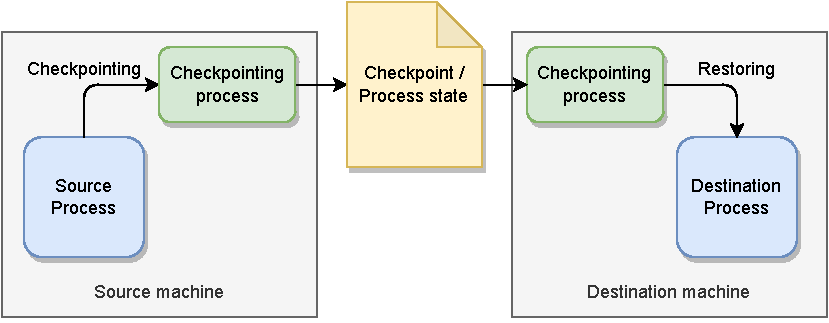
\includegraphics{images/process migration terminology.drawio-1.drawio-3.pdf}}
%\begin{verbatim}
%                      Process migration
%               ______________________________
%                
%                       (checkpoint or)
%                     ->(process state)-
%      checkpointing /                  \ restoring
%                    |                   V
%            (source process)      (destination process)
%    
%            [source machine]      [destination machine]
%\end{verbatim}

\caption{Conceptual visualization of process migration}
\end{figure}

\begin{itemize}[font=\textbf,leftmargin=2.7cm]
	\item[Process migration] is the act of checkpointing a process from the source machine and restoring this process on the destination machine~\cite{process-migration}. More information in \autoref{sec:process-migration}.
	\item[Source machine] is the machine we migrate from. On this machine, we only run our checkpointing tool. We do not tamper with the machine further.
	\item[Source process] is the process running on the source machine we want to checkpoint. This process is only temporarily suspended and copied, not altered.
	\item[Destination machine] is the machine that receives the process. We can shape it to our liking to match the source machine.
	\item[Destination process] is the process we create on the destination machine in which to restore the source process.
	\item[Checkpoint] is the process state as complete as possible to restore the process from this state. A checkpoint includes all the data we collect when checkpointing the source process. Ideally, this is the complete process state.
	\item[Checkpointing] is storing the process state to restart the process from this state. A good checkpointing implementation can migrate processes. More information in \autoref{sec:checkpointing}. Checkpointing is done on the source machine.
	\item[Restoring] is the method we use to restore the destination process from a checkpoint. This is done on the destination machine.
	\item[Checkpointing process] is the process we use to checkpoint the source process and restore the destination process. This process runs our implementation of process migration.
\end{itemize}

%\mainmatter

\chapter{Introduction}
\label{ch:introduction}
The world becomes more and more digital and we have become more reliant on the digital domain than ever before. This brings a lot of opportunities, but also raises the risk of digital attacks: malware can do more damage than ever~\cite{metro2023malware}.
Malware analysis is crucial for the detection and prevention of these digital attacks. There is an ongoing cat-and-mouse game between the malware writer and the analyst for better evasion of analysis and better analysis techniques.
For example, modern malware does all kinds of checks on startup to prevent dynamic analysis~\cite{al-khaser}, and some malware only resides in memory.
Dynamic analysis for this kind of malware can be very difficult.
Dynamic analysis of in-memory malware requires analysis on the infected machine, but this is not preferred, since we want to analyze in our quarantined malware lab.
We also may want to keep the malware running on the infected machine, to keep the forensic traces intact.
In this thesis, we aim to find out if it is possible to migrate a running process from one Windows 10 machine to another and research if this is useful for malware analysis. We choose this operating system because 83\% of malware is written for Windows~\cite{avtest2020report}.

To specify the goal of this thesis, our main research question is twofold and the two questions are as follows:

\begin{enumerate}[font=\textit,leftmargin=1.6cm,rightmargin=0.6cm]
	\item[RQ1:] \textit{Is it possible to migrate a running process from one Windows~10 machine to another machine?}
	\item[RQ2:] \textit{To what extent is process migration a useful method for the analysis of malware?}
\end{enumerate}
%\begin{quote}
%	\textit{RQ1: Is it possible to migrate a running process from one Windows~10 machine to another machine? }\end{sloppypar}
%\end{quote}
%
%\begin{quote}
%	\textit{RQ2: To what extent is process migration a useful method for the analysis of malware?}
%\end{quote}

In Windows, process migration is not a trivial task to achieve. Running a process from the start is trivial since this would only require us to load the correct program. But resuming a checkpointed process from where it left off is complex. It requires one to checkpoint the complete state of the process and restore a process in such a way it is almost the same as the original process, yet on a different machine. To achieve this goal, this thesis investigates the Windows operating system. We explain how processes are created, how memory is managed, and how handles work.

We incrementally work towards a solution. We begin by migrating a toy example consisting of two assembly instructions in \autoref{ch:shellcode}. This lays the foundation of our process migration. We extend our method by migrating all the memory of a process, or so-called virtual address space, in \autoref{ch:memory}. Then we extend our method by migrating the handles (e.g. file handles) of a process in \autoref{ch:handles}. Each step increases the complexity of our implementation. In every chapter, we demonstrate how to collect the process state to create a checkpoint and how to restore a process from a checkpoint.

`Migrating a Windows process' is a very broad research goal. To narrow this down, the scope we have is:
\begin{enumerate}
	\item Windows 10 only (version 22H2).
	\item x86-64-bit architecture.
	\item No GUI applications.
\end{enumerate}

Process migration is already complex enough without differences in Windows version and CPU architecture. Our method is Windows version dependent due to the use of internal structures and functions in Windows. Because of this, we further narrow our scope to a single version of Windows 10 and a single architecture. Because GUI applications also increase complexity, they are considered out of scope.

In our literature research (in \autoref{ch:related-work}) we find \textit{checkpointing} was indeed possible in 1999~\cite{chung1999winckp} for Windows NT on the same machine. However, the Windows OS has become a lot more complex over time, making this solution unusable for Windows 10 processes. In Linux, a few solutions exist already to migrate a process. However, current solutions for Windows are outdated or incomplete and in this research, we show process migration is indeed possible (up to a certain extent, more on this in \autoref{ch:conclusion}).

\section{Reading guide}
\label{sec:reading-guide}

In \autoref{ch:related-work}, we describe related work in the academic literature and existing software solutions.
We explain the related notions \textit{checkpointing}, \textit{process migration} and \textit{forking} and discuss how they relate to each other and our work. We describe existing solutions for Windows and Linux. 
Afterward, we describe related work in exploit development and fuzzing to describe their relation with process migration.

In \autoref{ch:shellcode} (toy example), \autoref{ch:memory} (memory), and \autoref{ch:handles} (handles), we describe our method to migrate different types of processes. Each with increased difficulty. Each chapter has the same structure. We describe how our migration method works and what we need for a proper checkpoint to store it all in a checkpoint file.
Later on, we describe how to restore a process from a checkpoint file and its workings. Finally, we verify our method.

In \autoref{ch:real-world} we verify whether we can migrate real-world malware and discuss possible showstoppers.
\autoref{ch:future-work} provides suggestions for future work. Finally, we conclude and reflect on our work in \autoref{ch:conclusion}. 


\chapter{Related work}
\label{ch:related-work}
% Database voor erg veel scientific papers, mocht het achter een paywall staan
% https://sci-hub.se/

The academic literature is widely available regarding process migration with other motivations~\cite{huang1998nt-swift}\cite{ansel2009dmtcp}\cite{barak1998mosix}\cite{khidhir2012migrationwin7}. For example, process migration is found in computing clusters to balance the computing load. Most of the research we find regarding checkpointing and process migration is with this goal in mind. The important difference between process migration in computing clusters and process migration in forensics is that computing clusters are designed to checkpoint and migrate processes whereas our environment and malware are not. Because of this difference, most process migration tools can record the state outside of the process and follow the process from startup. We are not able to accomplish this, since we miss the start of the source process.

We observe most of the research is done for the Linux kernel~\cite{ansel2009dmtcp}\cite{paul2006BLCR} and Virtual Machines as a whole~\cite{park2011checkpointing-vm}\footnote{\url{https://learn.microsoft.com/en-us/azure-stack/hci/manage/vm-load-balancing}}.
Windows is quite different from Linux, but we can learn from the methodology and design of a solution. Also, the limitations of a certain approach are interesting to note.

In the 1990s and early 2000s, there was more focus on computations in a cluster of machines. A lot of research has been done on checkpointing and process migration~\cite{barak1998mosix}\cite{ousterhout1988sprite}. Nowadays, the research for checkpointing for process migration on the process level subsided, but we observe a rise in practical open-source implementations~\cite{ansel2009dmtcp}\cite{criu}.

\textit{Forking} is a restricted form of checkpointing. \textit{Forking} can be described as checkpointing a process and immediately starting a new process with this checkpoint, creating a duplicate of the same process. We discuss \textit{forking} in Windows in more detail in \autoref{sec:checkpointing-in-windows}.

The next sections demonstrate what we can learn from the academic literature and how related applications work and relate to our research. We describe \textit{checkpointing} in Linux in \autoref{sec:checkpointing}. \autoref{sec:checkpointing-in-windows} describes \textit{checkpointing} and \textit{forking} in Windows. 
Related work around \textit{Process migration} can be found in \autoref{sec:process-migration}.
The section also describes the usage process migration done in computer clusters, fuzzing tools, and exploit writing.

With our gained knowledge we demonstrate our method to migrate processes in the next chapters. We start with a toy example in \autoref{ch:shellcode}.

\section{Checkpointing in Linux}
\label{sec:checkpointing}
Process \textit{checkpointing} is the method of creating a snapshot of the process' state, to roll back or restart from this state in case a crash or failure is imminent.
This use case overlaps with multiple other domains, for example, forensics, multiple node computing, and fault mitigation. Because of this, there are different terminologies for the same phenomena. 
\textit{Checkpointing} can also be called \textit{checkpoint/restore}, \textit{checkpoint/restart} and \textit{rollback recovery}. In this thesis, we will use the term \textit{checkpointing}. We distinguish two types of \textit{checkpointing}:
\begin{enumerate}
	\item A checkpoint is created by the process itself to store the data required for the current state. This is called a ``save state''. In this thesis, we are not interested in this type of \textit{checkpointing}.
	\item A checkpoint is created externally by a service that snapshots the process, such as a hypervisor snapshotting a VM\footnote{\url{https://docs.vmware.com/en/VMware-vSphere/7.0/com.vmware.vsphere.vm_admin.doc/GUID-9720B104-9875-4C2C-A878-F1C351A4F3D8.html}}. This method is called transparent checkpointing since the process does not know that a checkpoint was made.
\end{enumerate}

On Linux systems, a wide collection of solutions for \textit{checkpointing} is available. Solutions include: \textit{DMTCP}~\cite{ansel2009dmtcp}, \textit{CRIU}~\cite{criu}, \textit{BLCR}~\cite{paul2006BLCR},  \textit{Linux-CR}~\cite{laadan2010linux} and others~\cite{laadan2007transparent}\cite{zhong2001crak}. This is mostly due to the wide usage of Linux in the academic world and Linux is fully open-source. In the next subsections, we will describe some checkpointing implementations mentioned above in more detail. The implementations chosen all have a slightly different approach.

\subsection{DMTCP}
\label{sec:dmtcp}
Distributed Multi-Threaded CheckPointing (\textit{DMTCP})~\cite{ansel2009dmtcp} runs on Linux and transparently checkpoints a single-host or distributed computation in user space, with no modifications to user code or the OS.
As new processes are created, the \texttt{LD\_PRELOAD} environment variable is used to preload the \textit{DMTCP} library (\texttt{dmtcphijack.so}). This library runs before \texttt{main()} and does the following:

\begin{enumerate}
	\item It launches a checkpoint management thread in every user process.
	\item It adds a wrapper around a small number of \textit{libc} functions to record information about open sockets, etc. at creation time.
\end{enumerate}

\textit{DMTCP} does a shadow bookkeeping of open sockets and file handles to be able to ``replay'' data streams after a recovery. \textit{DMTCP} also uses the \texttt{/proc} file system to probe the kernel state. Their first publication is from 2006 and the last release is from 2019. However, their GitHub repository is still active in 2023.\footnote{\url{https://github.com/dmtcp/dmtcp}}

\textit{DMTCP}'s approach requires preloading their library during the start of a process. This means one has to deliberately start the process with \textit{DMTCP} to be able to checkpoint it in the future. Since the goal of our research is to avoid startup, this approach is not usable for our use case.

Alex Sardan~\cite{dmtcp-windows} started a \textit{DMTCP} clone for Windows. Although it compiles, restoring from a checkpoint does not work and is not complete in the current state. It seems to be a discontinued small hobby project. The code is available online and may serve as inspiration for others.

\subsection{BLCR}
\label{sec:blcr}
Berkeley Lab Checkpoint/Restart for Linux (\textit{BLCR}) is a checkpointing tool that uses a kernel driver to checkpoint processes~\cite{paul2006BLCR}. Instead of injecting threads in user space as \textit{DMTCP} does (described in \autoref{sec:dmtcp}), it uses a kernel module to follow the open sockets and used memory. They derive their code from a kernel module called \texttt{VMADump}~\cite{vmadump}. \texttt{VMADump} is a kernel module that saves or restores a process' memory space to or from a stream.
\textit{BLCR} does not support checkpointing important resources such as TCP/UDP sockets~\cite{paul2006BLCR}.
Their first release was in 2003~\cite{blcr}.
Kernel modules are quickly deprecated and outdated in newer kernel versions and thus need regular maintenance (as they discuss in their paper~\cite{paul2006BLCR}). Because of the higher maintenance, the project had its last update in 2013 and is no longer maintained.  
Kernel programming is more time-consuming, more challenging, and also more difficult to maintain than programming in user space. Because of that, we prefer to abstain from \textit{BLCR's} method.  
If our goal is not possible in user space, \textit{BLCR's} method may be suitable.

\subsection{Linux-CR}
\label{sec:linux-cr}
\textit{Linux-CR}~\cite{laadan2010linux} takes the approach of designing kernel drivers and syscalls to the checkpoint and restarting a process hierarchy, i.e. multiple processes in a hierarchy. The paper was written as a proposal for standardized checkpointing in the Linux kernel. Their method is to \textit{freeze} a tree of target processes and checkpoint all global data and states of all processes. Resources such as open files are also saved. Afterward, the processes are killed. Their checkpoint is stored in a file for it to be migrated or stored as a backup.
In the references section of this report, we find many examples of application checkpointing~\cites{paul2006BLCR}{zhong2001crak}{laadan2005commodity}{osman2003zap}. As described in the previous section, Since \textit{Linux-CR} makes use of a kernel module, we wish to abstain from \textit{BLCR's} method

\subsection{CRIU}
\label{sec:criu}
Checkpoint/Restore In Userspace, or \textit{CRIU} (pronounced kree-oo)~\cite{criu} can \textit{freeze} or checkpoint running Linux containers or standalone processes and save them to disk. The checkpoint procedure relies heavily on the \texttt{/proc} file system and the \texttt{ptrace} system call~\cite{criu}. The \texttt{/proc} file system acts as an interface to internal data structures in the kernel. It can be used to obtain information about the system and to change certain parameters at runtime.\footnote{\url{https://www.kernel.org/doc/html/latest/filesystems/proc.html}} With the \texttt{ptrace()} system call one process can observe and control the execution of another process, and examine and change the process' memory and registers. It is primarily used to implement breakpoint debugging and system call tracing~\cite{ptrace}. The resources are obtained via:

\begin{enumerate}
	\item Virtual memory areas are parsed from \texttt{/proc/\$pid/smaps} and mapped files are read from \texttt{/proc/\$pid/map\_files} links.
	\item File descriptor numbers are read via \texttt{/proc/\$pid/fd}.
	\item Core parameters of a task (such as registers and friends) are being dumped via \texttt{ptrace} interface and parsing the \texttt{/proc/\$pid/stat} entry.
\end{enumerate} 

Then \textit{CRIU} injects a parasite code into a process via the \texttt{ptrace} interface. This is done in three steps:
\begin{enumerate}
	\item At first we inject only a few bytes for an \textit{mmap} syscall at the instruction pointer when the task is at the moment of seizing. 
	\item Then \texttt{ptrace} allows us to run the injected syscall and we allocate enough memory for a parasite code chunk we need for dumping. 
	\item The parasite code is copied into a new place inside the dumper address space and the instruction pointer is set respectively to point to the parasite code.
\end{enumerate}

From this context \textit{CRIU} reads more information such as credentials and contents of memory.
\textit{CRIU} is currently used and is integrated into many container runtimes such as Docker\footnote{\url{https://docs.docker.com/engine/reference/commandline/checkpoint/}}, Podman\footnote{\url{https://podman.io/docs/checkpoint}}~\cite{htet2021podman-criu}, Kubernetes\footnote{\url{https://fosdem.org/2023/schedule/event/container\_kubernetes\_criu/}} and LXC\footnote{\url{https://linuxcontainers.org/lxc/manpages/man1/lxc-checkpoint.1.html}}.
\textit{CRIU} can also be used for process migration.

\textit{CRIU} seems to be the modern solution for checkpointing in Linux. \textit{CRIU} was initially released in 2012~\cite{criu}.
The latest release was in 2022, which shows us it is actively being developed.
We can learn what \textit{CRIU} stores in modern operating systems to create a proper checkpoint.
One might think \textit{CRIU} would be very useful for this research.
However, since \textit{CRIU} heavily relies on the \texttt{/proc} file system, which is not all available on Windows, we cannot use the same strategy. Another downside is that handles in Linux are very different compared to Windows, so we cannot use CRIU's approach with handles.
On the plus side, we can use the parasite code strategy to collect information not available from outside of the process. 

\section{Checkpointing in Windows}
\label{sec:checkpointing-in-windows}
In 1999, Chung, \textit{et al.} demonstrated a complete transparent checkpointing and recovery implementation on Windows NT~\cite{huang1998nt-swift}\cite{chung1999winckp}. They demonstrate \textit{Nt-SwiFT}: a collection of tools to build fault-tolerant and highly available applications on Windows NT. As the authors mention, the \textit{SwiFT} components were originally designed on UNIX, and are ported to Windows-NT. Their method of checkpointing a process is very similar to our method. The authors mention the usages of Windows API calls such as: \texttt{VirtualQueryEx} and \texttt{ReadProcessMemory}. \textit{NT-SwiFT} intercepts all Windows API calls which create file handles, process handles, thread handles, socket handles, and Windows handles. It also intercepts Winsock communication endpoints and logs messages. It even records mouse inputs and keystrokes. During recovery, \textit{NT-SwiFT} recreates the communication channels and replays all logged messages, keystrokes, etc.
They showed that even opened files and network traffic were restored and most processes could be restored flawlessly. Their website went offline years ago, but the Web Archive still has their website~\cite{web:winckp}. Unfortunately, the code and binaries are unavailable.
Nevertheless was \textit{Nt-SwiFT} of great use as inspiration for our method.

\subsection{Forking in Windows}
\textit{Forking} is an operation whereby a process creates a duplicate of the same process and that is executed afterward. This allows for concurrent programs. \textit{Forking} can be seen as a restricted form of checkpointing. It can be described as checkpointing a process and starting a new process with this checkpoint, creating a duplicate of the same process. The difference is a checkpoint can be stored on disk and a \textit{fork} immediately starts a new thread. Windows does not facilitate forking as a UNIX system does. We looked into forking implementations in Windows~\cite{cygwin}\cite{microsoft2016wsl}\cite{midipix}, but found them of little use.

%In the early days, Windows already supported Windows Services for UNIX (SFU) but was not updated anymore since 2004.\footnote{\url{https://en.wikipedia.org/wiki/Windows_Services_for_UNIX}}. The interesting part here is the \textit{fork} system call which is an operation that copies itself.
%\textit{fork} is an operation whereby a process creates a copy of itself. Everything is copied, like memory and thread context. This also includes memory and opened file handles. The \textit{fork} system call is found in UNIX/Linux environments. Windows does not have an implementation in user space for \textit{fork}, so to \textit{fork}, different libraries had to create one themselves.
%Since variables, etc. are copied over, this is a very useful mechanism for certain use cases. For example, the call is mainly used in shells like bash to run processes in the background.
%In this section we describe multiple implementations of forking in Windows and discuss their use in our research.
%
%Andrew Baumann, \textit{et al.}~\cite{baumann2019fork} As the designers and implementers of operating systems, they show us the problems that arise when implementing \textit{fork}. They claim of how \textit{fork} is not secure and is bad for performance, but these are not required in our research (up to a certain extent). Next to their warning us against using fork how it ``harms applications and OS design.'', we can conclude we are not affected by the problems they state, albeit being reassured implementing \textit{fork} is difficult. Luckily, \textit{Cygwin}'s implementation of \textit{fork} proves \textit{forking} is indeed possible on a Windows system as we show in the next section.
%
%\todo[inline]{ZwCreateProcess, ZwCreateUserProcess}
%
%\subsection{Cygwin's Fork}
%\label{sec:cygwin-fork}
%\textit{Cygwin}~\cite{cygwin} is a POSIX-compatible programming and run-time environment that runs natively on Microsoft Windows. Under Cygwin, source code designed for Unix-like operating systems may be compiled with minimal modification and executed. Due to the POSIX compliance, \textit{fork} is also implemented. Since we wish to copy a process, the internals of Cygwin's \textit{fork} are a great inspiration. The code is well-documented and can be found in their GitHub Repository~\cite{cygwin-fork}.
%
%Unfortunately Cygwin does its own memory management, it does not use the Heap manager provided by windows. Because of this, their way of copying the memory is unusable for process that use the normal heap manager.
%
%\todo[inline]{Zoek dit nog even verder uit: \url{https://cygwin.com/cygwin-ug-net/highlights.html\#ov-hi-process}}
%
%\subsection{Midipix's fork}
%Another POSIX-compatible programming and run-time environment for Windows is currently being developed, namely \textit{midipix}\todo{cite}. 
%% Unlike Cygwin, midipix widily uses the Windows Native API.
%Midipix's implementation for fork mainly uses the native function \texttt{ZwCreateUserProcess} to fork a process. 
%\footnote{\url{https://dev.midipix.org/runtime/ntapi/blob/main/f/src/process/ntapi\_tt\_fork.c}}
%
%% https://news.ycombinator.com/item?id=9651011
%
%% \subsection{Scilab's fork}
%% \label{sec:scilab-fork}
%% Probably for more readable multi-platform code, the open source software for numerical computation software \textit{Scilab} has developed their own \textit{fork}. What the system call \textit{fork} does is described in \autoref{sec:cygwin-fork}. The source code can be found in their Gitlab Repository~\cite{scilab-fork}. Their fork involves around \texttt{ZwCreateProcess}, setting the TEB(see \autoref{sec:TEB} and the thread starting point.
%
%\subsection{WSL's fork}
%\label{sec:wsl-fork}
%Current versions of Windows now have the possibility to run linux programs directly on Windows. This product is call Windows Subsystem for Linux, or \textit{WSL}. in Linux fork is available, so through WSL, fork may also be available to Windows.
%WSL executes unmodified Linux ELF64 binaries by emulating a Linux kernel interface on top of the Windows NT kernel~\cite{microsoft2016wsl}.
%The Linux \textit{fork} syscall has no documented equivalent for Windows. When a \textit{fork} syscall is made on WSL, kernel mode pico driver \texttt{lxss.sys} does some of the initial work to prepare for copying the process. It then calls internal NT APIs to create the process with the correct semantics and create a thread in the process with an identical register context. Finally, it does some additional work to complete copying the process and resumes the new process so it can begin executing.
%
%Unfortunately, we cannot use this work on normal processes, only pico processes. And since WSL's fork dives deep into the kernel and is quite vaguely documented~\cite{microsoft2016wsl}, this method is of little use for us.

\section{Process migration}
\label{sec:process-migration}
As shown in the previous checkpointing methods (\autoref{sec:checkpointing} and \autoref{sec:checkpointing-in-windows}), a well-designed checkpointing service can allow checkpointed processes to be restarted not only on their original machine but also on other machines that are supported.
\textit{Process migration} is the method of moving a running process from one machine to the other~\cite{process-migration}. \textit{Transparent} process migration means the process being copied does not know or notice it is being copied.
Process migration is preemptive: the process is already running and the state is saved and migrated to another machine. Non-preemptive process ``migration" is called process placement~\cite{krueger1988load}.
\looseness=-1

Khidhir \textit{et al.}~\cite{khidhir2012migrationwin7} described the design and implementation of process migration in Windows 7. Their paper describes technical terms which were useful for this thesis. Currently, this paper from 2012 is the most recent research for Windows on the subject we have found. Their method is similar to \textit{Nt-SwiFT}~\cite{huang1998nt-swift}, by making use of the same Windows API calls. An interesting difference is they use the PE header in the binary to restore certain parts of the memory. Their method is rather limited since they do not migrate any handles or log any messages. They only migrate memory, thread context, and binary. Nevertheless, their description of terms and their method was useful for the development of our implementation.
\looseness=-1

\subsection{Process migration in computing clusters}
Process migration is mainly used for distributed computing clusters to balance the computing load over the network and to prevent imminent crashes by migrating the process currently running on failing hardware~\cite{process-migration}.
At the end of the previous century, the academic field was actively developing operating systems that support the migration of processes. The operating systems were designed for computer clusters to distribute the load between machines with process migration. Some examples of these operating systems are: \textit{MOSIX}~\cite{barak1998mosix} and \textit{Sprite}~\cite{ousterhout1988sprite}.
\looseness=-1

\textit{MOSIX}~\cite{mosix} works as a software layer that allows processes to run in remote computers as if they run locally. The current version of \textit{MOSIX}~\cite{mosix} works on an unpatched Linux kernel. \textit{MOSIX} supports (preemptive) process migration among nodes in a cluster. Process migration consists of checkpointing the memory image and setting the run-time environment.
When a process is migrated, \textit{MOSIX} intercepts all system calls and forwards them to the source machine.
For every process, a mailbox is created which can receive and send messages to other processes in the cluster. These mailboxes work independently of the location of the process and allow for migratable sockets. In comparison to our scenario, forwarding all system calls to the source machine would not be desirable. This would defeat the whole purpose of the analysis.

% Generally process migration can be divided into two categories, Homogeneous and heterogeneous Homogeneous process migration means the underlying system will remain the same, eg. both systems are running Windows 11. Heterogeneous process migration is the movement of a process to a different underlying system, for example between a Windows system and an iPhone.

\subsection{Process migration in fuzzing}
\label{sec:related-other-uses}
Fuzzing is a form of automated testing and is the method of attempting many inputs on a program to find errors in the code. To improve performance, many fuzzing tools checkpoints just before the target function to save initialization time every round. The popular fuzzing tool called \textit{AFL}~\cite{afl} runs on Linux and uses a \textit{forking} server to \textit{fork} at the moment the process waits for input. \textit{AFL} is also ported to Windows and is called \textit{WinAFL}~\cite{winafl}. Unfortunately \textit{WinAFL} has a very rough approach of ``checkpointing'' by only moving the instruction pointer back to the start of the function that we want to fuzz. We conclude the fuzzing research is of little use to us since we require a more robust method.
% \todo{Vertel miss ook even welke toepassingen er voor Windows fuzzing nog meer zijn.}

\subsection{Process migration in exploit development}
\label{sec:software-security}
In exploit development, the malware creates processes to their liking in Windows.
Process injection in exploits uses many Windows API calls that are also useful for our implementation. Most of the time when process injection occurs, the shellcode is injected into a process. One of the properties of shellcode is that it works independently of its location in memory. More information about shellcode can be found in \autoref{sec:code-shellcode}. \textit{Meterpreter}~\cite{Meterpreter}, a popular shellcode from \textit{Metasploit}~\cite{Metasploit}, for example, has a command to inject itself inside another process. It copies its shellcode into memory and launches a thread to run the shellcode. Although this is related to process migration, inserting a process into another process is very different.

% \section{Conclusion}


% ======================== S H E L L   C O D E ========================

\chapter{Migrating a toy example}
\label{ch:shellcode}

In this chapter, we describe our method to migrate a process. We demonstrate this with the easiest process we could think of a toy program consisting of two assembly instructions: we increment a register and jump back to the start of the loop.
Our method of process migration takes place in three steps:
\begin{enumerate}
	\item Collecting the data of the state of the sourcing process to create a checkpoint (\autoref{sec:collecting-the-relevant-data}).
	\item Storing the collected data in a file called checkpoint.dat and moving it from the source machine to the destination machine (\autoref{sec:moving-shellcode}).
	\item Restoring the destination process from this checkpoint (\autoref{sec:restoring-checkpoint-shellcode}).
\end{enumerate}

\begin{figure}[h]
%\begin{verbatim}
%          ___________________   _________________________
%          |                  |  |                       |
%          | (source process) |  | (destination process) |
%          |        |         |  |         ^             |
%          |        V      2.moving        |             |
%          | 1.checkpointing----------->3.restoring      |
%          |                  |  |                       |
%          |_[source machine]_|  |_[destination machine]_|
%\end{verbatim}
\centerline{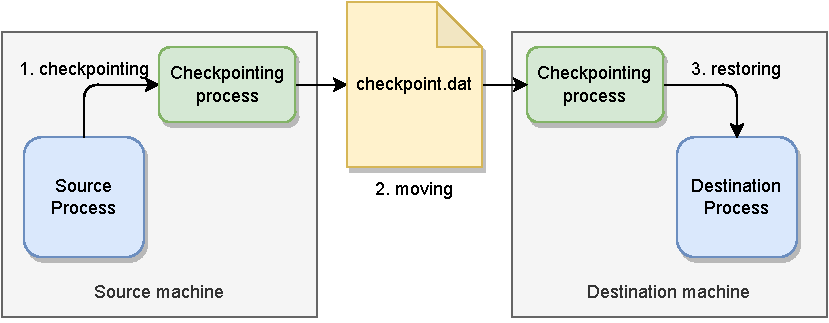
\includegraphics{images/process migration method.drawio-1.drawio-1.pdf}}
\caption{Flow of process migration}
\label{fig:flow-process-migration}
\end{figure}

\autoref{fig:flow-process-migration} shows a visual representation of process migration.
Step 2, moving the data, is a requirement that is trivial to perform. Steps 1 and 3 are the complex parts.

%\paragraph{Approach}
In this chapter, we only migrate a very simple process. As is also mentioned in \autoref{ch:introduction}, we work towards a solution incrementally. By consecutively adding components to migrate, we increase the complexity of each chapter step by step.
Every milestone has its chapter, and the structure of these chapters remains the same. We extend our processes with the following milestones:

\begin{enumerate}
	\item Thread context, i.e. CPU registers (this chapter).
	\item All process memory: memory pages, e.g. stack, heap, PEB, TEB, image file, and DLLs (see \autoref{ch:memory}).
	\item Handles, e.g. opened files, stdout, stdin, registry keys, and (network) sockets (see \autoref{ch:handles}).
\end{enumerate}

The source code of the complete implementation can be found on: \url{https://github.com/keukentrap/process-copy}.

We start by describing the background information required to understand what processes are in \autoref{sec:background-shellcode}. \autoref{sec:code-shellcode} describes our toy example.
\autoref{sec:collecting-the-relevant-data} discusses how all relevant data is collected on the source machine to create our checkpoint. \autoref{sec:moving-shellcode} describes the method of how to create a checkpoint file to send to the destination machine. \autoref{sec:restoring-checkpoint-shellcode} then discusses how to migrate our toy program. 

\section{Background: Processes}
\label{sec:background-shellcode}
In this section, we provide background information about processes and treads in Windows and provide information about the Windows API and its documentation.
\looseness=-1

\subsection{Difference between a program and a process}
\label{sec:program-vs-process}
To prevent further confusion, the terms program and process may seem to be interchangeable, but there is a difference.
\begin{description}%[font=\textbf,leftmargin=1.9cm]
	\item[Program] When we execute a program that is compiled, the OS creates a process to execute the program. A program is a passive entity that resides on a disk. One program can produce several processes.
	\item[Process] The term process refers to program code that is loaded into memory so it can be executed by the CPU. A process can be described as an instance of a program running on a computer. A program becomes a process when loaded into memory and is called an active entity.
\end{description}

\begin{figure}[h]
%	\begin{verbatim}
%                   file               memory
%                ___________         ___________
%                |PE Header|--\      |  ...    |
%                |---------|   \     |---------|
%                |Imports  |-\  ---->| PEB     |
%                |---------|  \      |---------|
%                |Sections |   |     |---------|
%                |.textbss |---+---->|Code     |
%                |.text    |   |     |---------|
%                |.data    |    \    |---------|
%                |   ...   |     --->|Ntdll.dll|
%                |_________|         |lib.dll  |
%                |   ...   |         |   ...   |
%                |_________|         |         |
%                
%                 [Program]           [Process]
%	\end{verbatim}
\centerline{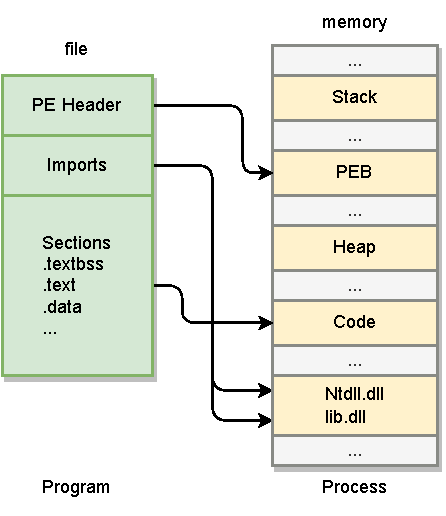
\includegraphics{images/program-vs-process.drawio.pdf}}
	\caption{Difference between a program and a process}
	\label{fig:program-vs-process}
\end{figure}

As we see in \autoref{fig:program-vs-process}, a program file contains the information and content to initialize a process.
More information about how a process starts from a program can be found in \autoref{sec:background-memory}.

\subsection{Threads and thread context}
Each process has one or more threads. Each thread has a Thread Environment Block (TEB) which contains thread-specific data. More on the TEB can be found in \autoref{sec:TEB}.

To create the illusion of running more threads simultaneously than CPU cores available, the CPU constantly switches between all running threads. During this multitasking, the thread context is constantly being loaded and stored. The thread context contains all the values of the registers of the CPU when the thread was suspended. To restore a process, all threads and their context also have to be restored.
The thread context contains essential information such as the instruction pointer. Without the thread context, resuming the migrated process would be impossible. To fully restore a process, all its threads have to be restored. In this chapter, we only consider single-threaded processes. In \autoref{ch:handles}, we add multi-threaded processes.

The x86-64 architecture has 16 general purpose 64-bit registers.\footnote{\url{https://learn.microsoft.com/en-us/windows-hardware/drivers/debugger/x64-architecture}} Some important registers to note are shown in \autoref{tab:registers}.

\begin{table}[h]
	\begin{tabular}{p{0.22\textwidth-2\tabcolsep} p{0.78\textwidth-2\tabcolsep} }
		\hline
		\textbf{Register} & \textbf{C/C++ compiler calling convention } \\
		\hline
		\textbf{rip} & is the instruction pointer and points to the next instruction that will be executed. \\
		\textbf{rsp} & is the stack pointer and points to the top of the stack. \\
		\textbf{rcx, rdx,} \newline \textbf{r8, r9} & are used to pass integer and pointer arguments to functions. Any additional arguments are pushed on the stack. \\
		\textbf{rax} & contains the return value of a function. \\
		\hline
	\end{tabular}
	\caption{Common registers and their function in x86-64}
	\label{tab:registers}
\end{table}

\subsection{Windows API}
The Windows API was formerly called Win32 API, but this was confusing as it roots in 16-bit Windows and also supports 64-bit Windows.\footnote{\url{https://learn.microsoft.com/en-us/windows/win32/apiindex/windows-api-list}} The Windows API contains a vast amount of functionality that runs on all versions of Windows. Our implementation makes use of many Windows API functions to collect data and restore a process.

A lot of useful information can be found in the official Microsoft documentation~\cite{win32-api}. In particular, the books called \textit{Windows Internals}~\cite{windows-internals}\cite{windows-internals-2} are of great help in learning the internals of Windows. When diving into the official documentation, one is likely to discover that some data structures (and functions) are missing. These are called ``opaque" data structures. They are not officially documented, since Microsoft wants to have the ability to alter them in the future and does not document them for better backward compatibility guarantees. In this research, we make a lot of use of these opaque data structures and not officially documented functions. So we risk our migration method may not work on future versions of Windows. Luckily, these opaque data structures are not unknown.
\looseness=-1

Software such as \textit{ReactOS}~\cite{reactos} and \textit{Wine}~\cite{winehq} can run Windows programs that use these data structures and have documented them. Multiple websites~\cite{undocumented}\cite{process-hacker-docs} have collected these undocumented functions and data structures. The official debugger called \textit{WinDbg}~\cite{windbg} is also an excellent tool for obtaining information about opaque data structures.
Last, write-ups for Windows exploits are useful for learning the technical details of the OS.\footnote{\url{https://www.ired.team/offensive-security/defense-evasion/finding-all-rwx-protected-memory-regions}}\footnote{\url{https://captmeelo.com/redteam/maldev/2022/05/10/ntcreateuserprocess.html}}

% Useful resource explaining process injection in Windows
%\url{https://resources.infosecinstitute.com/topic/poor-mans-process-migration-windows/}
%\url{https://decoder.cloud/}

\subsection{Sysinternals tools}
The Sysinternals tools are an official set of debugging tools for Windows. These tools are very useful to collect information about processes. For each process, it provides a list of used resources. \textit{Process Explorer}~\cite{process-explorer} is part of the Sysinternals suite and is a greatly improved task manager that displays a lot of information per process. Very similar tools, namely \textit{Process Hacker}~\cite{process-hacker}, and the recent successor \textit{System Informer}~\cite{system-informer}, also exist and show even  more information.

\section{The wrapper around our toy program}
\label{sec:code-shellcode}
We execute our toy program the same way one may execute shellcode. A shellcode is a small piece of code used as the payload in the exploitation of a software vulnerability. It is called ``shellcode" because it typically starts a command shell from which the attacker can control the compromised machine, but any piece of code that performs a similar task can be called shellcode.\footnote{\url{https://en.wikipedia.org/wiki/Shellcode}}
In our case, the shellcode is benign and is not launched via a vulnerability.

This toy program only consists of only two assembly instructions. The program loops indefinitely and increments a counter. The program only uses two registers (\texttt{eax} and \texttt{rip}) and a self-allocated memory page that is easy to checkpoint. Using this toy program has multiple benefits. This loop does not require any other memory pages such as the stack, heap, or other DLLs. The loop also does not need external handles, such as files or network streams. And the memory page does not require an absolute position in the Virtual address space and thus can be easily copied.
In order the launch our toy program, we have written a wrapper to launch this program, as shown in \autoref{lst:shellcode}.

\begin{lstlisting}[float=h,label=lst:shellcode,language={[Visual]C++},caption={The wrapper for our shellcode}]
#include<Windows.h>

// start:
//   inc eax    ; FF C0
//   jmp start  ; EB FC
const char toy_program[] = "\xFF\xC0\xEB\xFC";

int main()
{
	void *buf = VirtualAlloc(NULL, sizeof(toy_program), MEM_COMMIT | MEM_RESERVE, PAGE_EXECUTE_READWRITE);
	if (!buf) { return 1;}
	memcpy(buf, toyprogram, sizeof(toy_program));
	// Cast the pointer to a function pointer and run the toy program.
	(*(void (*)()) buf)();
}
\end{lstlisting}

Our toy program is currently located in the .data section in the binary. Because of a security measure called \textit{Data Execution Prevention (DEP)}, we cannot execute our program in the .data section. 
It has to be moved to a memory region where it can be executed. So we allocate a page and mark it as executable. \texttt{VirtualAlloc} does this on line 11 in \autoref{lst:shellcode}. On line 15, we run our toy program by first casting the buffer to a function.

\section{Collecting state to create a checkpoint}
\label{sec:collecting-the-relevant-data}
The goal of our checkpointing method is to collect all the data of the process state we need to migrate the source process.
In the following subsections, we show our checkpointing method for the toy program. We describe how every item in this list can be collected and copied. 
But first, we show the outline of our procedure to checkpoint the memory and thread context of our source process:


\begin{enumerate}
	\item Find the source process.
	\item Suspend threads of the source process.
	\item Checkpoint the relevant memory page (in this case only the toy program).
	\item Checkpoint thread context of the main thread.
	\item Resume threads.
\end{enumerate}

In order to create a checkpoint for our current example, we only have to checkpoint the memory page with our toy program and the thread context.
By looking for the protection \texttt{PAGE\_EXECUTE\_READWRITE} on the copied memory pages (as described in \autoref{sec:collecting-shellcode}), we find our needed memory page.
Since our toy program only uses two registers (the \texttt{eax} and \texttt{rip} registers) we only have to checkpoint these as the thread context (as described in \autoref{sec:collecting-thread-context}).

\subsection{Collecting the toy program}
\label{sec:collecting-shellcode}
We first have to find the source process. We can iterate over all processes with \texttt{CreateToolhelp32Snapshot}, \texttt{Process32First} and \texttt{Process32Next}. Note that the numbers 32 in the function names do not relate to 32-bit. 
With every iteration, we get information about a process, such as a process handle, its name, and the number of threads it has. This way we can find the process we want to migrate.

\begin{lstlisting}[float=h,label=lst:mem-pages,language={[Visual]C++},caption={Reading all memory pages from a process}]
MEMORY_BASIC_INFORMATION mbi;
LPVOID offset = 0;	
while (VirtualQueryEx(process, offset, &mbi, sizeof(mbi)))
{
	if (mbi.Protect == PAGE_EXECUTE_READWRITE 
	    && mbi.State == MEM_COMMIT)
	{
		curmem = new Memory;
		curmem->mbi = mbi;
		curmem->buf = new BYTE[mbi.RegionSize];
		memory_list->push_back(curmem);
		ReadProcessMemory(process, mbi.BaseAddress, curmem->buf, mbi.RegionSize, NULL);	
	}
	offset = (LPVOID)((UINT64)mbi.BaseAddress + mbi.RegionSize);
}
\end{lstlisting}

After we find our process, we run the code shown in \autoref{lst:mem-pages}. We loop over the virtual memory with \texttt{VirtualQueryEx}, storing the \texttt{MEMORY\_BASIC\_INFORMATION} (more information in \autoref{sec:memory-tranplanting-vm}) and checkpointing the contents of the page regions with \texttt{ReadProcessMemory}. As the name \texttt{ReadProcessMemory} implies, the function reads the virtual memory of a process starting from a given address until a given size. To support multiple memory pages, we save the memory pages in a list. For our current example, we filter for the protection \texttt{PAGE\_EXECUTE\_READWRITE} to get our toy program. This may include false positives, but it does not hurt to migrate those memory pages since they will not be used.
\looseness=-1

\subsection{Collecting thread context}
\label{sec:collecting-thread-context}
In Windows, the data structure called \texttt{CONTEXT}\footnote{\url{https://learn.microsoft.com/en-us/windows/win32/api/winnt/ns-winnt-context}} contains the thread context in 64-bit processes. The functions \texttt{GetThreadContext} and \texttt{SetThreadContext} can be used to get and set the thread context of a specific thread.

With calls to the functions \texttt{CreateToolhelp32Snapshot}, \texttt{Thread32First} and \texttt{Thread32Next} in the Windows API we can find the threads corresponding to our source process.
A single process may contain multiple threads that actually perform the execution.
And again, the number 32 in the function names does not relate to 32-bit. 

We can find the main thread by looking for the longest-living thread. We checkpoint the thread context of the main thread. In the checkpointing methods described in the next chapters, we also checkpoint the corresponding PEB and TEB addresses. More about the TEB is found in \autoref{sec:TEB}. In \autoref{ch:handles}, we checkpoint all threads.

\section{Moving our toy example}
\label{sec:moving-shellcode}
In the previous section (\autoref{sec:collecting-the-relevant-data}), we showed how to collect the process state. In this section, we describe how we store the collected data and we describe how we send it to the destination machine. First, we prepare the process for transmission by storing the complete state in a single file in \autoref{sec:storing-state}. Second, we send this file to our destination machine.

We started with migrating a toy program from and to the same machine. This lowered the complexity and improved development time. Later on, when we developed our checkpoint file, we found that migrating to another machine did not add more complexity.

As described in the introduction, we are allowed to modify the destination machine to our wishes.
A lot of the environment can be different when the process is migrated to another machine. Since our toy program is system-independent (only architecture dependent), we do not have to change anything on the destination machine.

\subsection{Storing a process' state in a single file}
\label{sec:storing-state}
We have defined a format to store the information collected in the previous two sections in a single file called: \texttt{checkpoint.dat}. The complete format can be found in \autoref{ap:fileformat}. For now, we add the following items to our checkpoint file.

\begin{enumerate}
	\item Thread context of main thread (\texttt{CONTEXT}\footnote{\url{https://learn.microsoft.com/en-us/windows/win32/api/winnt/ns-winnt-context}})
	\item Self-defined memory struct that contains the toy program:
		\begin{enumerate}
		\item \texttt{MEMORY\_BASIC\_INFORMATION}\footnote{\url{https://learn.microsoft.com/en-us/windows/win32/api/winnt/ns-winnt-memory_basic_information}}
		\item Content of memory page in bytes
		\end{enumerate}
	      
\end{enumerate}

With \texttt{fwrite} we write the content to a new file for every element in our file format.
Afterward, we send this file from the source machine to the destination machine.
\looseness=-1

\section{Restoring the checkpoint}
\label{sec:restoring-checkpoint-shellcode}

With our checkpoint file created in the previous section, we start to restore our destination process. With \texttt{fread} we read the contents of the process in the checkpoint file.
We start ``notepad.exe`` as a new process with \texttt{CreateProcessA} (can be any standard program). We do not want the process to start yet, so we start the process with its thread suspended (\texttt{CREATE\_SUSPENDED}).

% \todo[inline]{Mention this write-up: \url{https://www.ired.team/offensive-security/code-injection-process-injection/process-hollowing-and-pe-image-relocations}}

The current procedure to restore the process is as follows:
\begin{enumerate}
	\item Create a suspended process with \texttt{CreateProcessA}
	\item Allocate the page with \texttt{VirtualAllocEx} and write the contents with \texttt{WriteProcessMemory}.
	\item Set the thread context with \texttt{SetThreadContext}.
	\item Resume the main thread with \texttt{ResumeThread}.
\end{enumerate}

\section{Verification}
\label{sec:verification-shellcode}
In this section, we verify whether our migration succeeded by demonstrating the toy program is indeed running on the destination machine.
By attaching a debugger~\cite{x64dbg} and suspending the destination process, we can confirm the instruction pointer is pointing to our toy program. Here we can observe the \texttt{eax} register is incremented every cycle. We can also confirm in the Task Manager our process now utilizes 100\% of a single core, as expected.
From these observations we can conclude we are able to migrate toy programs.

% ============================ M E M O R Y ============================

\chapter{Migrating the virtual address space of a process}
\label{ch:memory}
In the previous chapter, we designed a source process without stack, without heap and without needing an executable image it was launched from. However, most processes are started from an executable file and use a stack and heap. To migrate these more complex processes we describe in this chapter how we migrate all the memory pages in the virtual address space from the source process to the same position in the destination process. To summarize, this includes the following items stored in memory:

\begin{enumerate}
	\item Stack
	\item Heaps
	\item Program image
	\item Loaded DLLs
	\item Process Environment Block (PEB) and related pages
	\item Thread Environment Block (TEB) and related pages
	\item All other pages that are allocated
\end{enumerate}

In this chapter, we briefly describe how all the components mentioned above work and describe their function. Furthermore, we demonstrate how these items can be collected and can be restored.

\autoref{sec:background-memory} describes the background information about memory management and program startup in Windows. \autoref{sec:collecting-memory} describes how to collect all memory pages in the virtual address space. \autoref{sec:moving-memory} describes what we append to the checkpoint file. \autoref{sec:memory-restoring-checkpoint} explains how to restore all memory pages from the checkpoint file. Finally in \autoref{sec:verification-memory} we verify whether a verification process can be successfully migrated.


\section{Background: Memory management}
\label{sec:background-memory}
In order to understand why and how our migration of memory works, we need background information about how Windows implements virtual memory. We describe the basic services provided by the memory manager and key concepts such as virtual memory and security measures such as \textit{ASLR} and \textit{DEP}. More detailed information can be found in the books ``Windows Internals"~\cite{windows-internals} and ``What Makes it Page?"~\cite{what-makes-it-page}.

%\begin{figure}[h]
%\begin{verbatim}
%                       __________________
%                       |USER_SHARED_DATA|
%                       |----------------|
%                       |...             |
%                       |----------------|
%                       |Stack           |
%                       |----------------|
%                       | PEB            |
%                       |----------------|
%                       |Heap            |
%                       |----------------|
%                       |Code            |
%                       |----------------|
%                       |----------------|
%                       |Ntdll.dll       |
%                       |lib.dll         |
%                       |   ...          |
%                       |________________|
%
%\end{verbatim}
%\caption{Schematic of virtual address space of a process.}
%\label{fig:virtual-memory}
%\end{figure}
%\todo{Hoe is deze weergave nuttig? Leg uit.}

\subsection{Memory Manager}
As the name suggests, the memory manager controls the memory in Windows. The memory manager is located in kernel space and has two primary tasks:
\begin{enumerate}
	\item Translating, or mapping, a process's virtual address space into physical memory. When a thread running in the context of that process reads or writes to the virtual address space, the correct physical address is referenced.
	\item Paging least used contents to disk if physical memory becomes sparse, also called swapping. Paging is irrelevant for us since the physical location of the data is not important.
\end{enumerate}

In this thesis, we focus on the former task, since we are not interested in where memory pages are stored in hardware. Only their virtual address and content are important.

\paragraph{Virtual and physical memory}
There is a difference between virtual memory and physical memory. As the term physical memory describes, physical memory has a physical address space, meaning an address points to a certain location in the RAM of a computer. Every process has its memory contained in a virtual address space. Virtual memory holds memory pages that the memory manager translates to a physical page stored in physical memory. An advantage of virtual memory is that processes can be isolated and are not able to read other processes' memory by default. Memory pages can be shared with other processes, as is the case with shared libraries for example.

\autoref{fig:memory-api} shows how all memory management APIs relate to each other. The Virtual API is the most low-level memory API we can use in user mode to allocate memory pages. In the next paragraphs, we describe these various APIs. The dotted box shows a typical C/C++ runtime implementation of memory management using functions, such as \texttt{malloc}, \texttt{free}, \texttt{realloc}, using the Heap API.
\looseness=-1

\begin{figure}[h]
%	\begin{verbatim}
%  [ Local/Global API (old) ]  [ C/C++ Runtime ]
%                 \                  /
%                  [    Heap API    ] 
%	                      |
%                  [  Virtual API   ]    [File Mapping API]
%   User mode                 \                   /
%   -----------------------------------------------------------
%   Kernel mode                 \               /
%                               [ Memory Manager ]
%\end{verbatim}
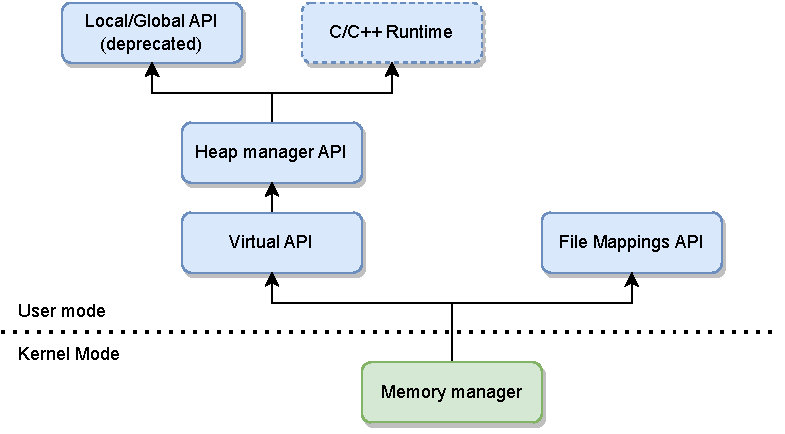
\includegraphics{images/MemoryAPI-3.drawio.pdf}
	\caption{Memory API groups in user mode.}
	\label{fig:memory-api}
\end{figure}

\paragraph{The Local/Global API}
are old and deprecated memory manager functions. Starting with 32-bit Windows (Windows 95), \texttt{GlobalAlloc} and \texttt{LocalAlloc} are implemented as wrapper functions that call \texttt{HeapAlloc} using a handle to the process' default heap.\footnote{\url{https://learn.microsoft.com/en-us/windows/win32/memory/comparing-memory-allocation-methods}}

\paragraph{The Stack manager}
The stack manager allocates the stacks for threads. The TEB contains information about the stack such as initial size and maximum size. The stack manager is fairly simple: on thread creation, the stack is initialized and memory is allocated. The stack grows from high to low. At a certain moment when the stack keeps growing in size, the stack exceeds its allocated size, and a page fault is hit. Since a stack is located on the memory page above it, the memory manager allocates an extra memory region for the stack. The stack never shrinks in size.

\paragraph{The File Mapping API}
projects the content of a file in the virtual address space. This allows for files to be used by file pointers pointing to virtual memory. This also allows files to be opened at once by multiple processes and for files to be lazily loaded. This is done by loading the contents from the disk when a page hit occurs. This paper will not be using this API.
We use the Virtual API to checkpoint file mappings.

\paragraph{The Heap manager}
manages the heaps for a process. The heap manager is made to allocate small areas with a granularity of 8 bytes (depending on the OS version) and large areas (\textgreater508~KB). The heap manager has been designed to optimize memory usage and performance in the case of these smaller allocations~\cite [p.332]{windows-internals}. How the heap manager works is a complicated subject. We will not go into too much detail for brevity. What is important to know is that there are different kinds of heaps: NT heap, low-fragmentation heap, and segment heap. Also, security features are implemented to detect simple corruptions to mitigate potential heap-based exploits~\cite[p.402]{what-makes-it-page}. Metadata is stored alongside heap allocations or at the start of the memory page, depending on the heap type. 

The heap manager uses the Virtual API (\texttt{VirtualAlloc}, etc.) under the hood to make its allocations. This means we can now utilize the Virtual API to checkpoint all heaps.
When we checkpoint the pages, the global metadata and the metadata for every heap are also copied. We adjust the fields in the PEB that relate to the heap, to let the heap manager know where our heaps are. More information about what is migrated can be found in \autoref{sec:PEB}.

\subsection{The Virtual API}
\label{sec:virtual-api}
is the most low-level API to manage memory~\cite[p.309]{windows-internals}. With this API, we can query, allocate, and free memory pages. A single memory page is 4KB. We use this to allocate our memory pages.
Some functions related to the Virtual API have \texttt{Ex} at the end. \texttt{Ex} is abbreviated from \texttt{Extension}. The extension for the Virtual API functions means that a process can query and allocate memory in other processes, not just its process memory.

With \texttt{VirtualQueryEx}\footnote{\url{https://learn.microsoft.com/en-us/windows/win32/api/memoryapi/nf-memoryapi-virtualallocex}} we query memory information about a specified address range of pages from the source process. This information contains for example whether the virtual memory is mapped to real memory and what its permissions are: read, write, and/or execute.\footnote{\url{https://www.ired.team/offensive-security/defense-evasion/finding-all-rwx-protected-memory-regions}} 
\texttt{VirtualQuery(Ex)} queries a region of pages if all these statements hold: 
\begin{enumerate}
	\item The state of all the pages is the same. (\texttt{MEM\_PRIVATE}, \texttt{MEM\_IMAGE}, \texttt{MEM\_MAPPED}, \texttt{MEM\_RESERVED}, \texttt{MEM\_COMMIT})
	\item The pages are allocated by the same \texttt{VirtualAlloc}, \texttt{MapViewOfFile} or their extended versions.
	\item The protection on all pages is the same. (\texttt{PAGE\_READ}, \texttt{PAGE\_READWRITE}, \texttt{PAGE\_EXECUTE\_READWRITE}, etc.)
\end{enumerate}

With \texttt{VirtualAlloc(Ex)}, we can allocate pages. We can reserve free pages, commit reserved pages, and reserve and commit free pages.
When allocating memory, we can distinct pages in three modes:
\begin{enumerate}[font=\texttt,leftmargin=2.7cm]
	\item[MEM\_RESERVED] The pages are reserved without any physical storage being allocated. The pages do not contain any data and protection is undefined.
	\item[MEM\_COMMIT] The pages are committed to physical memory, either in memory or in the paging file on disk. 
	\item[MEM\_FREE] The pages are not used and are free to be allocated.
\end{enumerate}

\subsection{When a process starts}
\label{sec:when-a-process-starts}
Multiple process-creation functions exist, but eventually result in calling the Windows API function \texttt{CreateProcessInternalW}. Later on, we will call this function \texttt{CreateProcess*}.
The flow of \texttt{CreateProcess*} consists of seven stages~\cite[p. 130]{windows-internals}:
\begin{enumerate}
	\item Converting and validating parameters and flags.
	\item Opening the image to be executed.
	\item Creating the Windows executive process object.
	\item Creating the initial thread and its stack and context.
	\item Performing Windows subsystem-specific initialization (out of scope).
	\item Starting execution of the initial thread.
	\item Performing process initialization in the context of the new process.
\end{enumerate}

To summarize these stages:
Stage 1 sets process attributes such as a possible debug mode. Stage 2 loads the binary file into memory and detects the type of program: a batch script, a legacy Windows application, or a regular executable. In this thesis, we only consider the last option: a regular executable. At stage 3 the process is created: a Windows executive process object is created in kernel space. The \texttt{EPROCESS} struct is created in kernel space and the PEB is created in user mode. In stage 4 the initial thread and its stack and context are created.  The TEB is allocated. We ignore stage 5 since Windows subsystem processes are out of scope.

Since we create a process with the \texttt{CREATE\_SUSPENDED} flag, our method pauses at stage 6. Stage 7 will mainly load the \texttt{Ntdll.dll} library and starts its initialization routine called \texttt{LdrInitializeThunk}. \texttt{LdrInitializeThunk} is responsible for initializing the image loader, the heap manager, and more structures. It then loads any required DLLs. Afterward, more structures are initialized but are omitted for brevity. A more detailed description of these stages can be found in ``Windows Internals Part 1''~\cite{windows-internals}. 

\subsection{Structure of a process}
\label{sec:process-structure}
A process is an instance of a program that is being executed by one or more threads. In Windows, every process has its own virtual address space (memory). The details about a process are mainly stored in two structs, one resides in kernel mode and the other in user mode.  
A process allocates in kernel mode an \texttt{EPROCESS} struct. \texttt{EPROCESS} is an opaque structure, meaning Windows does not officially document it. Since the \texttt{EPROCESS} is in kernel mode, a user in user mode is not able to edit the values inside the struct. The struct contains information such as Creation time, PID, and PEB address. It also contains various kernel-related information for a process.\footnote{\url{https://www.nirsoft.net/kernel_struct/vista/EPROCESS.html}}
A process also has a similar data structure in user mode, called the PEB. More info about the PEB can be found in \autoref{sec:PEB}.

\subsection{Import Address and Lookup table}
The Import Address Table is located in the PE header of the binary and contains entries for every DLL that is loaded by the executable. The Import Address Table is identical to the Import Lookup Table until the binary is loaded into memory. During binding, the entries in the import address table are overwritten with the 64-bit addresses of the symbols that are being imported.\footnote{\url{https://learn.microsoft.com/en-us/windows/win32/debug/pe-format?redirectedfrom=MSDN\#import-address-table}} Since these entries are set when a DLL or executable is loaded, the DLL or executable needs to be put in the same location as it was located.

\subsection{Windows API library \textit{Ntdll}}
\textit{Ntdll} is the native Windows library and comprises many user-mode Windows API functions. User-mode applications use the native system services routines by calling the functions in the \texttt{Ntdll.dll} library.\footnote{\url{https://learn.microsoft.com/en-us/windows-hardware/drivers/kernel/libraries-and-headers}} As described in \autoref{sec:when-a-process-starts}, \texttt{Ntdll.dll} is loaded in every process during process startup in stage 7.


\section{Collecting memory pages}
\label{sec:collecting-memory}
In this section, we describe how to collect all the memory used by a single process. The source process has its own virtual address space to store its data. More background information about the virtual address space can be found in \autoref{sec:background-memory}.

In \autoref{sec:collecting-the-relevant-data} we have shown how to find the process and collect the memory pages. In the previous chapter, we only checkpointed \texttt{PAGE\_EXECUTE\_READWRITE} memory pages. Now we checkpoint all memory pages regardless of protection. We checkpoint all reserved and committed pages. We also checkpoint the reserved pages to create allocations with the correct size. We collect all memory pages, as they are all possibly relevant to the process. The new step is marked in bold. The procedure is now as follows:

\begin{enumerate}
	\item Find the source process.
	\item Suspend threads of the source process.
	\item \textbf{Checkpoint all memory pages.}
	\item Checkpoint thread context of the main thread.
	\item Resume threads.
\end{enumerate}


\section{Moving the memory of a process}
\label{sec:moving-memory}
The complete format can be found in \autoref{ap:fileformat}. Compared to the previous chapter, we extend our checkpoint file with the following: 

\begin{enumerate}[]
	\item All memory pages: their \texttt{MEMORY\_BASIC\_INFORMATION} and their content.
	\item The Process Environment Block (PEB).
	\item The Thread Environment Block (TEB) for the main thread.
\end{enumerate}

The PEB and TEB are stored twice: once in the list of all memory pages and once separately. This is done for easier reference. The method of moving the memory of a process remains essentially and is described in the previous chapter (in \autoref{sec:moving-shellcode}). 

\section{Restoring the checkpoint}
\label{sec:memory-restoring-checkpoint}
Compared to the previous migration method, we have extended the second step by now migrating all memory pages. The new steps are marked in bold and will be discussed in the next subsections. The current procedure is as follows:

\begin{enumerate}
	\item \textbf{Create a suspended process of \texttt{Empty.exe} with \texttt{CreateProcessA}.}
	\item \textbf{Execute process initialization before main().}
	\item \textbf{Kill threads created by the Windows API library \textit{Ntdll}}.
	\item \textbf{Allocate and restore all memory in the correct position.}
	\item \textbf{Adjust the PEB.}
	\item \textbf{Adjust the TEB.}
	\item Set the thread context.
	\item Resume the main thread.
\end{enumerate}

More information about the newly added procedures mentioned above can be found in the next subsections.
In the previous chapter, we created a process running notepad.exe. For improved consistency, we now have written a special binary we start, namely \texttt{Empty.exe}. As the name may reveal, this program does nothing but loop infinitely, as shown in \autoref{lst:empty}.

\begin{lstlisting}[float=h,label=lst:empty,language={[Visual]C++},caption={All code of \texttt{Empty.exe}}]
void main() {
	while(true){}
}
\end{lstlisting}

\subsection{Impact of Address Space Layout Randomization (ASLR)}
\label{sec:aslr}
To prevent an attacker can predict an offset into either the program code or a DLL, \textit{Address Space Layout Randomization (ASLR)} was invented. ASLR randomizes the virtual starting address of the executable, thread stacks, heaps, and DLLs. At the start of every process creation, the executable, thread stacks, and heap starting addresses are randomized. For DLLs, the load offset is set during boot. This means the DLL starting address is random for every boot cycle, so during this boot cycle, the starting addresses for DLLs are the same in every process.
The existence of ASLR is important for process migration, since reminiscent heaps, stack, executables, and binary from `\texttt{Empty.exe}' will most likely be in another location than those from the destination process. The same holds for DLLs being located at a different address when we migrate to another machine. This is positive since collisions will be unlikely due to ASLR.

\subsection{Initialization before \texttt{main()}}
\label{sec:memory-main}
From the perspective of a programmer, one may think a process starts at \texttt{main()}. But before \texttt{main()} is called, many other functions already have been executed. This initialization is an important procedure for processes to function properly. To trigger this initialization, we resume the main thread and wait for a few seconds to suspend all the threads of our destination process again. 
This initializes the essential components in step 7 from \autoref{sec:when-a-process-starts}.
In our case, an important step is to run the image-loader initialization routine in \texttt{Ntdll.dll}, as well as the system-wide thread startup stub in \texttt{Ntdll.dll}~\cite[p. 149]{windows-internals}.
What is executed here in Windows is largely undocumented and differs per Windows version. By trial and error, we found out that running everything before the main gave a more stable process migration resulting in fewer unexpected crashes. 
Also, we discovered we are now able to attach a debugger to migrated processes, causing the analysis of crashes to be a lot easier.

\subsection{Kill threads created by the Windows API library \textit{Ntdll}}
\label{sec:killing-threads-memory}
During the initialization mentioned in the previous section, \textit{Ntdll} creates a thread pool of worker threads in our process. These worker threads allocate heaps, and this creates a problem. When those heaps are freed after we have restored them to the new heap manager, the process crashes. After debugging and reverse engineering the crash with IDA Pro~\cite{ida-pro}, we found out the segment code in the metadata of the heap is now invalid, resulting in a panic. To make sure a crash does not happen, we kill all worker threads before we restore the heap manager. This way we prevent the heap frees from happening after we restore the heap manager. Otherwise, the process will crash after several seconds.
\looseness=-1

\subsection{Restoring the virtual address space}
\label{sec:memory-tranplanting-vm}
Memory must be restored on the same addresses. As one would expect, quite some operations require the absolute address of data in memory. Some examples:
\begin{enumerate}
	\item Absolute jumps and external function calls require code to be in the same address.
	\item The call stack requires the functions that have been called to be on the same address.
	\item Pointers store the absolute address of the value they point to.
\end{enumerate}
The items mentioned above are critical to making execution work. So we need to restore the virtual address space and its content as accurately as possible. To achieve this goal, we have to understand the workings of the virtual address space.
\looseness=-1

\begin{lstlisting}[float=h,label=fig:mbi,language={[Visual]C++},caption={Struct of \texttt{MEMORY\_BASIC\_INFORMATION}}]
typedef struct _MEMORY_BASIC_INFORMATION {
   PVOID  BaseAddress;
   PVOID  AllocationBase;
   DWORD  AllocationProtect;
   WORD   PartitionId;
   SIZE_T RegionSize;
   DWORD  State;
   DWORD  Protect;
   DWORD  Type;
} MEMORY_BASIC_INFORMATION, *PMEMORY_BASIC_INFORMATION;
\end{lstlisting}

\texttt{VirtualQueryEx} returns a \texttt{MEMORY\_BASIC\_INFORMATION} struct. In \autoref{fig:mbi}, the fields of \texttt{MEMORY\_BASIC\_INFORMATION} are shown.\footnote{\url{https://learn.microsoft.com/en-us/windows/win32/api/winnt/ns-winnt-memory_basic_information}}
Next to the size, protections, etc., it contains two starting addresses: \texttt{BaseAddress} and \texttt{AllocationBase}. 
\texttt{BaseAddress} contains the start of the region of pages.
\texttt{AllocationBase} contains the base address of a range of pages allocated by the VirtualAlloc function.
These two values may be different, as shown in \autoref{fig:virtual-allocation}. We describe why in the next paragraph.

\begin{figure}[h]
%\begin{verbatim}
%            ...00000   -- |--|  <- AllocationBase
%                1000    - |XX|  <- BaseAddress
%                2000    - |XX|
%                3000    - |  |
%                4000    - |XX|  <- BaseAddress
%                5000    - |  |
%                ...       |  |
%                F000    - |__|
%            ...10000   --
%               11000    -
%                ...
%\end{verbatim}
\centerline{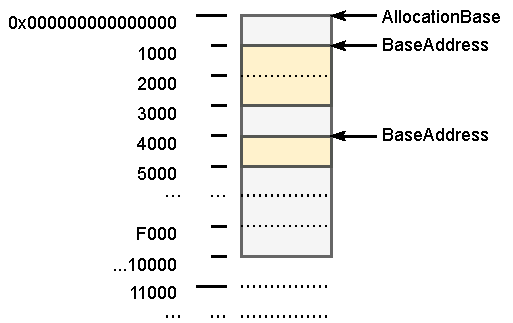
\includegraphics{images/memory-allocation.drawio.pdf}}
\caption{Visual representation of a memory allocation.}
\label{fig:virtual-allocation}
\end{figure}

Reserving memory with \texttt{VirtualAlloc} has to obey the allocation granularity. The allocation granularity in Windows 10 (and almost every other version of Windows) is 64KB (0x10000 bytes)~\cite[][p.107]{what-makes-it-page}. This means pages can only be reserved on addresses that align with this 64KB granularity. To allocate a page region inside this granularity (eg. a \texttt{BaseAddress} ending with 0x4000), we will start reserving at 0x0000. \texttt{VirtualAlloc} will align us to 0x0000. Luckily Windows itself also has to obey this rule, meaning all allocations have this alignment and thus can be restored. (all except USER\_SHARED\_DATA, more on this in \autoref{sec:user-shared-data}) 

To allocate and restore all memory in the correct position, we first reserve the page regions that share the same \texttt{AllocationBase}. This is done in the following steps: 
\begin{enumerate}
	\item Compute the required region size by finding the last page region with the same \texttt{AllocationBase} and computing: \texttt{TotalRegionSize} = \texttt{BaseAddress} - \texttt{AllocationBase} + \texttt{RegionSize}.
	\item Reserve page regions with \texttt{VirtualAllocEx}.
	\item Commit all page regions to memory for every page region we copied with \texttt{VirtualAllocEx}.
	\item Write the contents to memory with \texttt{WriteProcessMemory}.
	\item Set the correct protection with \texttt{VirtualProtectEx}.
\end{enumerate}

With this procedure, we can completely recreate the virtual address space of the source process.

\paragraph{3rd party DLLs}
\label{sec:implementation-dlls}
Many processes use libraries to access the functionality of the operating system. DLLs are used for modularization of code. Standard libraries such as \texttt{Ntdll.dll} are available on every Windows system. However, not every library will be available, so we have to migrate these as well. Migrated DLLs function without extra configuration: by migrating the memory because we also migrate the contents of the DLLs. 

Due to ASLR (\autoref{sec:aslr}), standard libraries will be put in a different address than if they normally would be loaded with \texttt{LoadLibrary}. This is not a problem since the process expects the library to be available at the exact address it was loaded.
\looseness=-1

\subsection{Adjusting the Process Environment Block (PEB)}
\label{sec:PEB}
The Process Environment Block (or PEB for short) is a data structure containing information about a process, including global context, startup parameters, data structures for the program image loader, and the program image base address. The PEB is a partially opaque data structure and is located in the virtual address space of the process itself. 
The PEB contains all kinds of process-specific data. For example, the \texttt{WindowTitle} is stored in the PEB. The definition of the PEB can be found online.\footnote{\url{https://www.vergiliusproject.com/kernels/x64/Windows\%2010\%20|\%202016/2110\%2021H2\%20(November\%202021\%20Update)/\_PEB}}

At this stage of the restoration, the current PEB is largely incorrect, since the newly created one (from \texttt{Empty.exe}) is still used.
Because the PEB Address is stored in the \texttt{EPROCESS} struct stored in kernel space, we cannot point to the migrated PEB. However, we can write to the newly created PEB and change its contents. In exploit development, this method is also called \textit{PEB masquerading}~\cite{peb-masquerading}. In this section, we show how we alter the PEB to reflect the PEB of the source process.

We modify as many fields as possible, only skipping the fields that relate to machine-related values, e.g. the number of CPU cores available.
We adjust the following fields in the PEB:
\begin{enumerate}
	\item \texttt{ProcessParameters} (includes \texttt{WindowTitle}, \texttt{Environment} variables)
	\item \texttt{ImageBaseAddress}
	\item Heap manager fields (\texttt{ProcessHeap}, \texttt{HeapSegmentReserve},\\ \texttt{HeapSegmentCommit}, \\ \texttt{HeapDeCommitTotalFreeThreshold}, \texttt{HeapDeCommitFreeBlockThreshold}, \texttt{NumberOfHeaps}, \texttt{MaximumNumberOfHeaps}, \texttt{ProcessHeaps})
	\item \texttt{LoaderData}
	\item \texttt{KernelcallbackTable}
	\item \texttt{UsersharedInfoPtr}
	\item \texttt{Apisetmap}
	\item Thread local storage fields (\texttt{Tlsbitmap}, \texttt{Tlsbitmapbit},\\ \texttt{TlsExpansionBitmap}, \texttt{TlsExpansionBitmapBits})
	%\item \texttt{ReadonlySharedMemoryBase} and \texttt{ReadonlySharedMemoryData}
	\item \texttt{Ansicodepagedata}, \texttt{Oemcodepagedata} and \texttt{Unicodepagedata}
%	\item \texttt{pShimData}\footnote{\url{https://techcommunity.microsoft.com/t5/ask-the-performance-team/demystifying-shims-or-using-the-app-compat-toolkit-to-make-your/ba-p/374947}}
%	\item \texttt{ActivationContextData}
%	\item \texttt{SystemdefaultContextData}
%	\item Thread pool fields (\texttt{Tppworkerlist})
\end{enumerate}
%\todo{Deze waslijst naar een Appendix?}

The most important adjustments are the fields related to the heap manager.
After these adjustments to the PEB, the PEB now points to the migrated heap.
The process now uses the migrated heap manager for future allocations and migrated heaps are recognized and fully usable. 

We also set the process-wide environment variables. Thread local storage fields are set as these may contain essential information.
The other fields are more of a nicety and set fields such as the program name and description. 

% https://www.wikiwand.com/en/Process_Environment_Block

\subsection{Adjusting the Thread Environment Block (TEB)}
\label{sec:TEB}
Every thread has a Thread Environment Block (TEB). The Thread Environment Block (TEB) is a data structure that contains thread-specific data. The definition of the TEB can be found online.\footnote{\url{https://www.vergiliusproject.com/kernels/x64/Windows\%2010\%20|\%202016/2110\%2021H2\%20(November\%202021\%20Update)/\_TEB}}
As with the PEB, we cannot point to the migrated TEB, we have to adjust fields in the newly created TEB.
We adjust the fields related to our scope and that are not related to the machine. What we do not adjust is the PEB address field, since we have not moved the PEB (see \autoref{sec:PEB}).
We change the following fields in the TEB:
\begin{enumerate}
	\item Stack related fields (\texttt{StackBase}, \texttt{StackLimit}, \texttt{DeallocationStack})
	\item \texttt{EnvironmentPointer}
	\item Thread Local Storage related fields (\texttt{ThreadLocalStoragePointer},\\ \texttt{TlsSlots}, \texttt{TlsExpansionSlots}, \texttt{TlsLinks})
	\item \texttt{HeapData} 
%	\item Fiber Local Storage related fields (\texttt{FlsData})
	\item Network related fields (\texttt{ActiveRpcHandle}, \texttt{WinSockData})
%	\item \texttt{pShimData}
%	\item Thread pool fields (\texttt{ThreadPoolData})
\end{enumerate}

The TEB currently points to the old stack. By adjusting this, our restored stack now acts as a stack and automatically grows when needed.
We also set the thread-specific environment variables. Thread local storage fields are set as this storage may contain essential information. Network-related fields are set to make networking possible in the future.

%\todo{meer uitleg, waarom dingen wel en waarom niet?}

\section{Verification}
\label{sec:verification-memory}
We have designed a program that uses the stack and heap to verify whether our migration succeeded and that the destination process is working as expected on the destination machine.
The program shown in \autoref{lst:memory-verification} makes use of the stack (\texttt{recursive}), the heap (\texttt{calloc}), and a global variable (\texttt{sleep}). We also make use of the \textit{Ntdll} function \texttt{Sleep}. As we observe the output shown in Figure \autoref{fig:memory-comparison}, we notice that the output of both processes is the same. Even the random seed is restored.

\begin{lstlisting}[label=lst:memory-verification,language={[Visual]C++},caption={The program to verify memory}]
#include <Windows.h>
#include <stdio.h>
#include <time.h>

int sleep;

int recursive(int i,char* p) {
	p[i] = '!' + i;
	if (i > 0) {
		return recursive(i - 1,p);
	}
	else {
		Sleep(sleep);
		return 1;
	}
}

int main()
{
	char* p;
	sleep = 3000;
	srand(time(0));

	while (1) {
		p = (char*)calloc(1000,sizeof(char));
		int i = rand() % 94;
		recursive(i,p);
		printf("%s\n",p);
		free(p);
	}
}
\end{lstlisting}

\begin{figure}[h]
\centerline{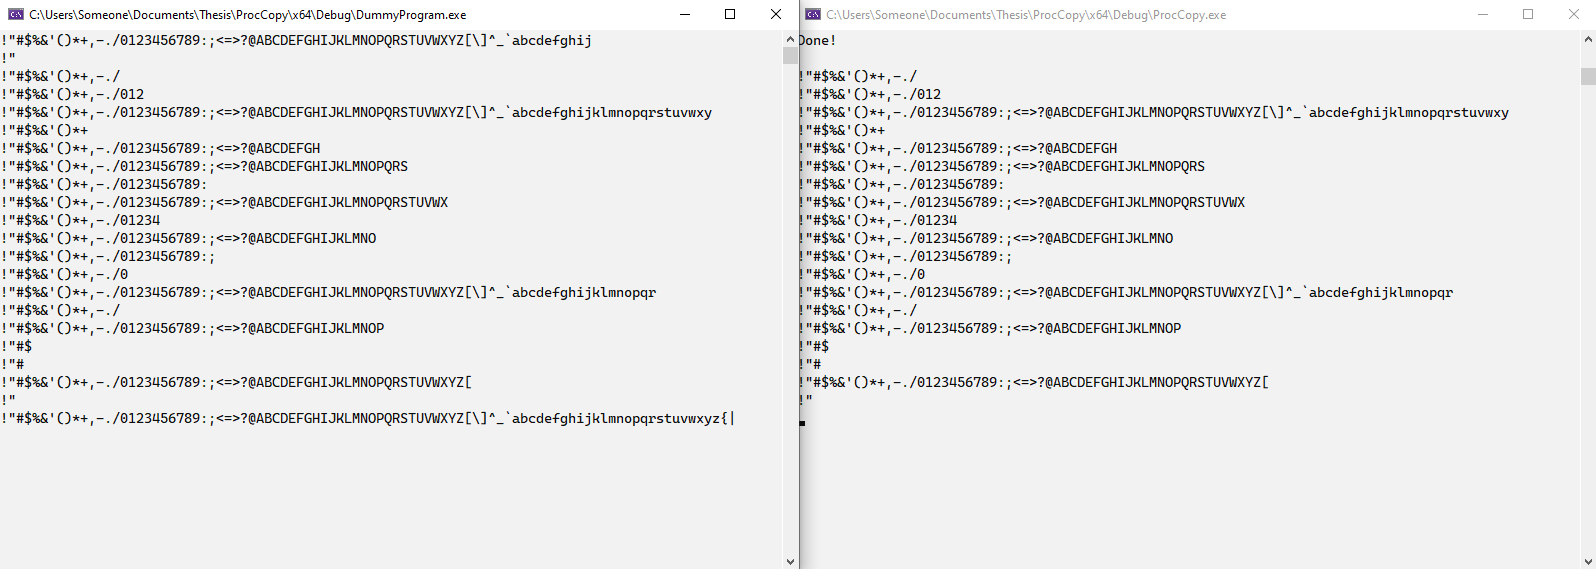
\includegraphics[width=1.2\textwidth]{images/memory-comparison-white.png}}
\label{fig:memory-comparison}
\caption{The output is the same on the two processes, even when a random seed was set. As expected, the destination process is slightly behind.}
\end{figure}

\subsection{What still goes wrong in memory}
\label{sec:memory-what-goes-wrong}

\paragraph{USER\_SHARED\_DATA}
\label{sec:user-shared-data}
At almost the start of the virtual address space, we find the page regions: 0x7ffe0000 and around 0x7ffe2000 to 0x7ffef000. These two regions contain the \texttt{USER\_SHARED\_DATA} and \texttt{HYPERVISOR\_SHARED\_DATA}.\footnote{\url{https://learn.microsoft.com/en-us/windows-hardware/drivers/ddi/ntddk/ns-ntddk-kuser\_shared_data}}
Both contain various information such as the system time and process architecture. The pages are read-only and their protection cannot be altered. This means we are not able to restore these pages. Another interesting (and trivial) phenomenon is that the second page (around 0x7ffe2000 to 0x7ffef000) has an \texttt{AllocationBase} not aligned to 64KB.

\paragraph{File mappings} What we may foresee as a problem in our process migration is that file mappings, such as DLLs, are not allocated by the file mapping API but by the Virtual API. We were warned this could be a problem, but we have not found this to be an issue.

% =========================== H A N D L E S ===========================
\chapter{Migrating a process that uses external resources}
\label{ch:handles}
Besides thread context and virtual memory, we also have to take into account the context outside of the process, such as opened files and network streams. Windows uses \textit{handles} to communicate with such resources. In this chapter, we show how the most common handles can be migrated. In particular: file handles, console handles, events, mutexes, and semaphores. This chapter builds upon the work in \autoref{ch:shellcode} and \autoref{ch:memory}. In the next chapter (\autoref{ch:real-world}) we test our final implementation on real-world malware.

We first provide background information about handles and how they are managed in \autoref{sec:background-handles}. \autoref{sec:collecting-handles} describes how to collect the handles from a process and \autoref{sec:moving-handles} describes what we add to our checkpoint file. \autoref{sec:handles-restoring-checkpoint} explains how to restore the handles we have checkpointed. At last, we verify whether our method works by migrating a test process in \autoref{sec:verification-handle}. As \autoref{sec:multithreading} we describe how to migrate multiple threads. 

\section{Background: handles}
\label{sec:background-handles}
Windows implements an object model to provide consistent and secure access to the various internal services implemented in the operating system. In this model, objects are managed by the object manager, which is responsible for creating, deleting, protecting, and tracking objects~\cite[p.125]{windows-internals-2}.
Windows has about 69 object types~\cite[p.128]{windows-internals-2}. %TABLE 8-15
In \autoref{fig:handles}, we provide a summarized overview of the available object types.

\begin{table}[h]
\begin{tabular}{p{0.22\textwidth-2\tabcolsep} p{0.78\textwidth-2\tabcolsep} }
\hline
\textbf{Object Type} & \textbf{Represents} \\
\hline
File & An instance of an opened file or an I/O device, such as a pipe, socket, or console \\
Event & An object with a persistent state that can be used for synchronization or notification. A global key is used to reference an event. \\
Semaphore & A counter that provides a resource gate by allowing a maximum number of threads to access the resources protected by the semaphore.\\
Mutex & A synchronization mechanism used to serialize access to a resource. \\
Key & A reference to a registry key. Although shown in the object manager namespace, it is managed by the configuration manager. A key contains zero or more values. \\
Section & A region of shared memory (known as a file-mapping object in Windows).\\
Process & The virtual address space and control information of a certain process. This also could refer to the process itself.\\
Thread & An executable entity within a process.\\
\hline
\end{tabular}
\caption{Some different types of handles. Other handles are omitted for brevity and are described in Windows Internals 7 Part 2~\cite{windows-internals-2}}
\label{fig:handles}
\end{table}

\begin{figure}[h]
%\begin{verbatim}
%         user space      |      kernel space
%         Process A       |
%                         |   
%                 Handle  |   Process A
%             (reference  |   handle table   
%               eg. 0x20) |  _______             
%                    |    |  |_____|          
%                    \------>|_____-->  object 
%                         |  |_____|           
%                         |  |_____|  
%                         |
%\end{verbatim}
\centerline{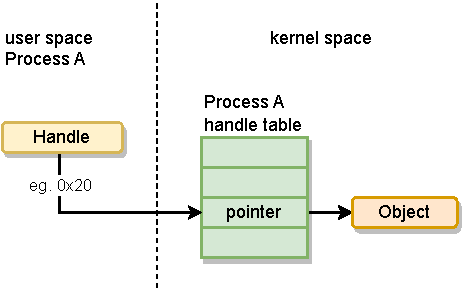
\includegraphics{images/handle-table.drawio-3.pdf}}
\caption{Process handle table}
\label{fig:process-handle-table}
\end{figure}

Every process has a handle table to maintain a list of its objects. This handle table (shown in \autoref{fig:process-handle-table}) contains references to the respective objects. The handle table resides in kernel space and is referenced by the \texttt{EPROCESS} struct (described in \autoref{sec:process-structure}). Every entry in the handle table contains an object reference along with its permissions and flags such as inheritance of the object to child processes~\cite{windows-internals-2}. 

\section{Collecting handles}
\label{sec:collecting-handles}
As described in \autoref{sec:background-handles}, a handle is an index in the handle table to another object pointer. Simply copying the handle table to migrate the handles would not suffice for two reasons. First, checkpointing the handle table would require a kernel driver on the source machine. Second, we cannot copy the object pointed to in the handle table, since they are bound to the components outside the process, e.g. files on the machine. We could write a kernel driver to retrieve the information about each object, but since kernel programming is more time-consuming and more challenging, we wish to abstain from developing one.
\looseness=-1

Instead, we opt for reconstructing the components outside of the process. By collecting as much information about an object as possible, we aim to reconstruct it as correctly as possible. We cannot always create a one-to-one copy of the external object, because not all information about an object can be collected or can be restored perfectly.
More about these shortcomings can be found in \autoref{sec:showstoppers}.
\looseness=-1

On the same machine, we can duplicate handles from one process to another using the Windows API in user mode.
With \texttt{NtQuerySystemInformation} we can query all handles in the system. By iterating over them and matching the process ID, we can get a list of handles from our source process. With \texttt{DuplicateHandle} we can duplicate these handles to our checkpoint process for further inspection.\footnote{\url{https://cplusplus.com/forum/windows/95774/}} With \texttt{NtQueryObject} we can query general information about the object behind the handle, in particular:
\begin{enumerate}
	\item Handle no.
	\item Type of handle
	\item Name (if given)
	\item Granted Access
\end{enumerate}

To correctly reconstruct the underlying object, we require more information. Which information depends on the handle type. In the next subsections, we describe how to collect information about specific handle types.


\subsection{Collecting information about files}
To migrate a file, we need to collect the handle, the file content, and the location inside the file.
Different file types exist.
With \texttt{GetFileType}\footnote{\url{https://learn.microsoft.com/en-us/windows/win32/api/fileapi/nf-fileapi-getfiletype}} we can differentiate between a disk file (a regular file), console stream, socket/pipe unknown handles. In this thesis, we focus on regular files and console handles.

With \texttt{NtQueryObject} we obtain a file path that corresponds to the handle. This function returns the file path in \textit{Logical Pathing Format}. Effectively this means that `\texttt{C:\textbackslash\textbackslash}' is renamed to `\texttt{\textbackslash device\textbackslash...}'. The Microsoft documentation\footnote{\url{https://learn.microsoft.com/en-us/windows/win32/memory/obtaining-a-file-name-from-a-file-handle}} gives a method to translate from logical pathing to the pathing format we can use, also known as \textit{Universal pathing}.

To properly restore a file handle we need to obtain the position in the opened file. A specific function to get this position does not exist. However with \texttt{SetFilePointerEx} and giving it a relative distance of 0 it returns the current position.\footnote{\url{https://learn.microsoft.com/en-us/windows/win32/api/fileapi/nf-fileapi-setfilepointerex}}
Finally, we read the contents of the file with \texttt{ReadFile}. We are now able to collect all the information we need to restore a file handle.
%\todo[inline]{\url{https://github.com/winsiderss/systeminformer/blob/29b9573667cfb869819ae30e56d24aaea73064a9/phlib/filestream.c\#L167}}
%\todo[inline]{\url{https://learn.microsoft.com/en-us/windows-hardware/drivers/ddi/ntifs/nf-ntifs-ntqueryinformationfile}}

\subsection{Collecting console handles}
Console handles are used to print to standard output and read from standard input. 
We can find in the PEB whether the console handle is standard input, output, or error. 

\subsection{Collecting information about events, mutexes and semaphores}
Mutexes and semaphores are both synchronization primitives designed for concurrency control~\cite{dijkstra1968structure}. To collect information about a mutex, we use \texttt{WaitForSingleObject} to acquire ownership and set the timeout to 1 ms. If the mutex is not yet acquired by another thread, we get the mutex and learn it was not yet acquired. Otherwise, we time out and learn the mutex is owned by another thread. If we acquired the mutex, we release the mutex afterward with \texttt{ReleaseMutex}.
 
To collect the current count and the maximum count of a semaphore, we use the \texttt{NtQuerySemaphore}\footnote{\url{https://undocumented-ntinternals.github.io/UserMode/Undocumented\%20Functions/NT\%20Objects/Semaphore/NtQuerySemaphore.html}} function to retrieve this information. We are now able to collect enough information about mutexes and semaphores. However, the mutexes and semaphores may be used by other processes we do not migrate. This may result in incorrect behavior since the mutex or semaphore will never be released.


\section{Moving the handles of a process}
\label{sec:moving-handles}

In this section, we move the handles, as described in \autoref{sec:collecting-handles}, to our destination machine. The complete format can be found in \autoref{ap:fileformat}.
We extend our format with the following. 

\begin{enumerate}
	\item Array with object information per handle (type, granted access, name, and more info per handle type).
\end{enumerate}

\section{Restoring the checkpoint}
\label{sec:handles-restoring-checkpoint}

The list shown below describes our final method to restore the destination process.
The new step is marked in bold and will be discussed in the next subsections. We set the handle table before the process initialization (see \autoref{sec:handle-setting-table}). This is because the process initialization before \texttt{main()} fills the handle table with other handles, which will prevent us from setting the handles in the correct location. The procedure is as follows:

\begin{enumerate}
	\item Create a suspended process with \texttt{CreateProcessA}.
	\item \textbf{Set the handle table}.
	\item Execute process initialization before \texttt{main()}.
	\item Kill threads created by the Windows API library \textit{Ntdll}.
	\item Allocate and restore all memory in the correct position.
	\item Adjust PEB and TEB.
	\item Set the thread context.
	\item Resume the main thread.
\end{enumerate}

\subsection{Setting the Process' handle table}
\label{sec:handle-setting-table}
As described in \autoref{sec:background-handles}, handles are merely pointers to addresses in the process' handle table.
We cannot assign a handle to a preferred address.
Luckily handle addresses are predictable. The addresses are incremented by 4 for every new handle, which is quite obvious since an object reference is a 32-bit integer and 4x8 = 32.
By creating every handle in the correct order, and adding ``filler'' handles, we can assign every handle to the correct address.

Every resource is first created and initialized in the checkpoint process. Then we move the handle over with \texttt{DuplicateHandle} to the destination process. The initialization of the resources is described in the next subsections.

% \todo[inline]{\url{https://rayanfam.com/topics/reversing-windows-internals-part1/}}

\subsection{Restoring files}
\label{sec:handles-file-handles}

The \texttt{CreateFile} function can open (or create) files and returns a handle. Before duplicating this handle, we write the content of the file with \texttt{WriteFile} and set the position in the file correctly with \texttt{SetFilePointer}.

\subsection{Restoring console handles}
\label{sec:handles-console-handles}
As is the case with our destination process, the console handles are inherited from our checkpointing process. The console handles will be at the beginning of the handle table. Modern console handles can be duplicated.\footnote{\url{https://github.com/rprichard/win32-console-docs/blob/master/README.md}} By duplicating an inherited corresponding console handle we can put the console handles in the correct position.

One downside of this method is that handles at the beginning of the handle table cannot be restored because the inherited console handles will be taking up their location.

\subsection{Restoring events, mutexes, and semaphores}
\label{sec:handles-other-handles}

The creation of events is done with \texttt{CreateEvent}. We create mutexes with \texttt{NtCreateMutant} and semaphores with \texttt{NtCreateSemaphore}.
Note that the events will be of little use since there is no other process or thread at the other end to receive from or send to. This may also be the case with mutexes and semaphores, since they are only used by the destination process, and not by any other process. 

Handles that we are currently not able to migrate are restored as an event with the type of handle as the name, as a surrogate. An example of this can be found in \autoref{fig:handle-comparison}.

\section{Verification}
\label{sec:verification-handle}
To verify whether all handles are correctly migrated, we have written a program shown in \autoref{lst:handle-verification} that uses the handle we have implemented: file handles, console handles, events, mutexes, and semaphores.

The program creates a mutex and semaphore. In an infinite loop, it opens a file on the desktop and asks for user input. Then it acquires the semaphore and mutex, prints a part of the content of the file, and releases both the semaphore and the mutex. Afterward, the file is closed and the loop starts over again.

\clearpage

\begin{lstlisting}[label=lst:handle-verification,language={[Visual]C++},caption={Our program to verify handles}]
#include <Windows.h>
#include <stdio.h>

#define FNAME "C:\\Users\\Someone\\Desktop\\Test2.txt"

int main(void)
{
    FILE* stream;
    HANDLE mutex = CreateMutex(0, true, L"TEST_Mutex");
    HANDLE semaphore = CreateSemaphore(0, 15, 15, L"TEST_Semaphore");
    char list[105]{};

    while (1) {
        if (fopen_s(&stream, FNAME, "rb") == 0)
        {   
            printf("enter position: ");
            int pos = 0;
            scanf_s("%d", &pos);
            fseek(stream, pos, SEEK_CUR);

            ZeroMemory(list, 100);
            fread(list, sizeof(char), 100, stream);

            WaitForSingleObject(mutex, 0);
            WaitForSingleObject(semaphore, 0);
            for (int i = 0; i < 100; i++) {
                printf("%c", list[i]);
            }
            ReleaseSemaphore(semaphore, 1, 0);
            ReleaseMutex(mutex);
            printf("\n");

            Sleep(200);
            fclose(stream);
        }
    }
}
\end{lstlisting}

After migrating this process, we can observe in \textit{System Informer}~\cite{system-informer} the handles of both the source process and destination process (as shown in \autoref{fig:handle-comparison}. The handles we migrated are correct and in the correct location. A file named ``\texttt{Test2.txt}'' is created on the desktop. By interacting with the destination process, we confirm that the console handles are functional on the destination process and work as expected.

\clearpage % otherwise the figure below disappears..

\begin{figure}[h]
	
	\centerline{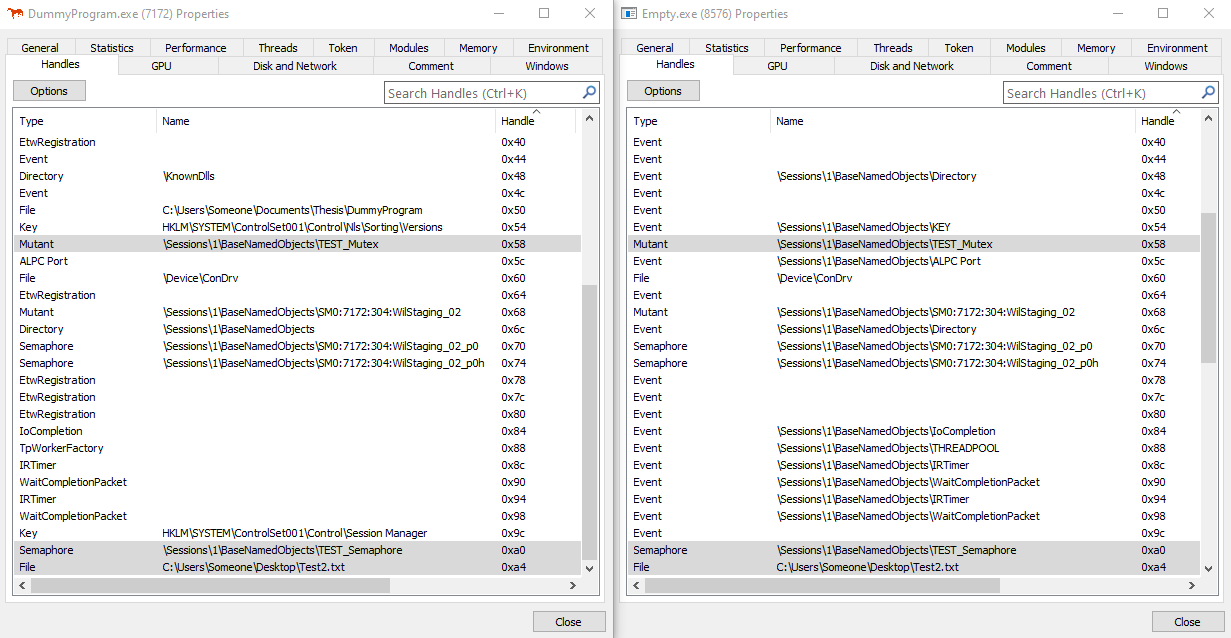
\includegraphics[width=1.2\textwidth]{images/handle-comparison-2.png}}
	\caption{Sample of handles from both processes. The source process is on the left, destination process is on the right.}
	\label{fig:handle-comparison}
\end{figure}

\section{Migrating a process with multiple threads}
\label{sec:multithreading}
Since we are now able to migrate mutexes and semaphores, multithreading is a logical addition.
We collect the thread context for every thread instead of only the main thread. During restoration, we recreate all threads and set the thread context for each of them. This way we support multi-threaded processes.


% =========================== M A L W A R E ===========================
\chapter{Migrating real-world malware}
\label{ch:real-world}
In this chapter, we use our implementation on real-world malware samples to validate our research.
We try to migrate \textit{Turian} malware designed for 64-bit Windows systems. We also tried to migrate Shadowspad malware, but this was deemed too hard to analyze. Later on in this chapter, we describe what can be done in principle and what fundamental showstoppers are in our process migration.
\looseness=-1

%\section{Migrating ShadowPad malware}
%In this section we verify whether it is possible to migrate ShadowPad malware. ShadowPad is publicly known malware developed by the BRONZE ATLAS threat group since 2017.\footnote{\url{https://www.secureworks.com/research/shadowpad-malware-analysis}} The malware is designed for 64-bit Windows machines. We have download our version from Virustotal\footnote{\tiny{\url{https://www.virustotal.com/gui/file/284c664b4baff90444c4ed96cfcb4ef6d26cc7aedc46c1e996c359ecea95f697}}} and the sha256 hash  is: \\
%\texttt{284c664b4baff90444c4ed96cfcb4ef6d26cc7aedc46c1e996c359ecea95f697}
%
%\todo[inline]{Describe more info about the malware.}
%
%\todo[inline]{Describe what goes wrong}

% \section{Ketrum2 malware}
% \todo[inline]{\url{https://www.virustotal.com/gui/file/aacaf0d4729dd6fda2e452be763d209f92d107ecf24d8a341947c545de9b7311/detection}}

\section{Migrating Turian Malware}
\label{sec:turian}
\textit{Turian} malware is attributed to the Chinese advanced persistent threat group called Playful Taurus, also known as APT15. The group routinely conducts cyber espionage campaigns. The group has been active since at least 2010 and has historically targeted government and diplomatic entities across North and South America, Africa, and the Middle East~\cite{turianmalware2023}.

In June 2021, ESET reported~\cite{backdoordiplomacy2023} that this group has upgraded its arsenal with a new backdoor called \textit{Turian}. We have downloaded a sample from Virustotal\footnote{\tiny {\url{https://www.virustotal.com/gui/file/6828b5ec8111e69a0174ec14a2563df151559c3e9247ef55aeaaf8c11ef88bfa}}} and the sha256 hash is: \\ 
\texttt{6828b5ec8111e69a0174ec14a2563df151559c3e9247ef55aeaaf8c11ef88bfa}

To migrate the malware, we first start the sample and observe its behavior. Since the sample is in the form of a DLL, we start the malware with \texttt{Rundll.exe}. As we observed, the malware creates a service called \textit{AppMgmt}. This service is then started and to connects to the C2 server located at \texttt{mail.indiarailways[.]net} at intervals.
\looseness=-1

When we migrate the process, we can observe the destination process contains all the correct memory pages. We also find two threads with the correct call stack, but when we resume the destination process, the process immediately crashes. By attaching the debugger from \textit{Visual Studio}~\cite{visual-studio} before we resumed the destination process, we get the following error message immediately after resumption:
\looseness=-1

\begin{verbatim}
(ImageAtBase0x7ff878480000) in Empty.exe: 0xC0020043:
  An internal error occurred in RPC  (parameters: 
  0x0000000000000002, 0xFFFFFFFFC0000024).
\end{verbatim}

In the call stack shown by the \textit{Visual Studio} debugger, we find the following function that caused the crash: \texttt{LRPC\_CASSOCIATION::AlpcCancelMessage()}. When we look at the handles created by the event, we see a special ALPC port handle, with the name: \texttt{\textbackslash RPC Control\textbackslash LRPC-c40de8e9f52c6a8bc3}. ALPC ports are used for inter-process communication. We do not migrate ALPC port handles, so closing a non-existing ALPC port will result in a crash.

\section{What can be done in principle?}
As we conclude in the previous section, our implementation is a start for process migration. In this section, we discuss what does not work in our implementation but can theoretically be done in practice. In the following sections, we gradually increase the complexity we estimate for every improvement.


%We can order these in 4 categories of complexity
%
%\begin{enumerate}[]
%	\item straightforward. The issue can be solved in user mode with ease.
%	\item kernel mode required. The issue needs to be resolved in kernel mode. This will add complexity since developing a kernel driver requires more technical skill and effort.
%	\item external party required. More is needed to be migrated, such as: other parties related to a resource (see \autoref{sec:other-end}).
%\end{enumerate}

\subsection{Resolving that a library is loaded twice}
At the creation of every process, the native Windows API library called \textit{Ntdll} is loaded (see \autoref{sec:when-a-process-starts}). The \textit{Ntdll} library is also migrated into a restored process, resulting in two versions of \textit{Ntdll} being loaded into memory: the migrated and the freshly loaded version. Important process state is stored inside this library. The migrated \textit{Ntdll} will have this state, but the freshly loaded \textit{Ntdll} will not. The problem is the OS/kernel will use the functions of the freshly loaded \textit{Ntdll}, resulting in a missing process state. As we have seen in our experiments, this results in unexpected behavior and mostly crashes. By hooking every function in the freshly loaded \textit{Ntdll} with the migrated \textit{Ntdll}, one can prevent the ambiguous state.

\subsection{Files and registry keys that are accessed after restoration}
It is imaginable that a process created a configuration file, closes the file, and reopens the file again after a while. When the file is not open during migration, we do not migrate the file. We can solve this by migrating every file in the system possibly on an on-demand basis. The same holds for registry keys.


\subsection{Migrating a wider range of handle types}
As mentioned before, our process migration does not support the complete range of handle types. We expect that by adding support for a wider variety of handles, it will become possible to migrate even more complex processes. Registry keys, named pipes, and thread handles are common handles in malware and can be restored as shown in \autoref{fig:future-handles}.

\begin{table}[h]
\begin{tabular}{p{0.22\textwidth-2\tabcolsep} p{0.78\textwidth-2\tabcolsep} }
\hline
\textbf{Object Type} & \textbf{Represents} \\
\hline
Registry key & Can be restored with \texttt{RegCreateKeyExA}.\footnote{\url{https://learn.microsoft.com/en-us/windows/win32/api/winreg/nf-winreg-regcreatekeyexa}} \\
Named pipe & A pipe for inter-process communication. Can be restored with  \texttt{CreatePipe}.\footnote{\url{https://learn.microsoft.com/en-us/windows/win32/api/namedpipeapi/nf-namedpipeapi-createpipe}} \\
ALPC Port & A method for inter-process communication used internally by Windows. Can be restored with \texttt{NtAlpcCreatePort} and \texttt{NtAlpcConnectPort}.\footnote{\url{https://csandker.io/2022/05/24/Offensive-Windows-IPC-3-ALPC.html}} \\
%Section & A region of shared memory (known as a file-mapping object in Windows).\\
Thread & An executable entity within a process. By collecting every thread ID first and translating those, the handle can be restored with \texttt{OpenThread}.\footnote{\url{https://learn.microsoft.com/en-us/windows/win32/api/processthreadsapi/nf-processthreadsapi-openthread}}\\
\hline
\end{tabular}
\caption{Migratable handle types, with varying complexity}
\label{fig:future-handles}
\end{table}

\subsection{Some handles require both a sending and receiving party to be restored}
\label{sec:other-end}
In \autoref{ch:handles}, we describe that it is seldom possible to create a one-to-one copy of everything on the handle. For some handles, it will be possible to restore all functionality, as is the case with normal file handles. But as with events, for example, this may be a showstopper. As shown in \autoref{fig:missing-end}, the other end of the events is currently not restored. One could restore the missing process with a mock-up, but this will not restore the complete functionality. Handle types that fall under this category are: events, mutexes, semaphores, named pipes, ALPC ports, and network sockets

\begin{figure}[h]
	\centerline{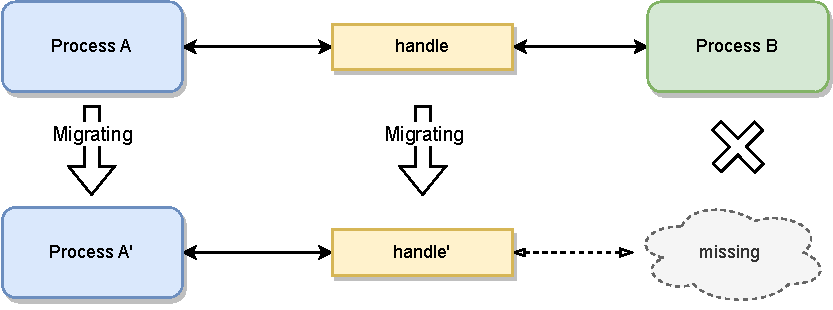
\includegraphics[width=\textwidth]{images/missing other end.drawio.pdf}}
	\label{fig:missing-end}
	\caption{The current implementation does not also migrate other processes or drivers that utilize the same resource.}
\end{figure}

\subsection{Restoring networking functionality}
\label{sec:handles-network-handles}
The main difficulty in migrating processes that use networking is the required initialization with \texttt{WSAStartup}. Windows networking operates via the \textit{Winsock2} networking driver. We can migrate all states inside the process, but we cannot migrate the state in the Winsock driver in the kernel. As we can see in \autoref{fig:networking} and depicted with a 1, the state inside the networking driver is not migrated. We propose that developing a kernel driver to modify the Winsock driver will solve this issue.

\begin{figure}[h]
	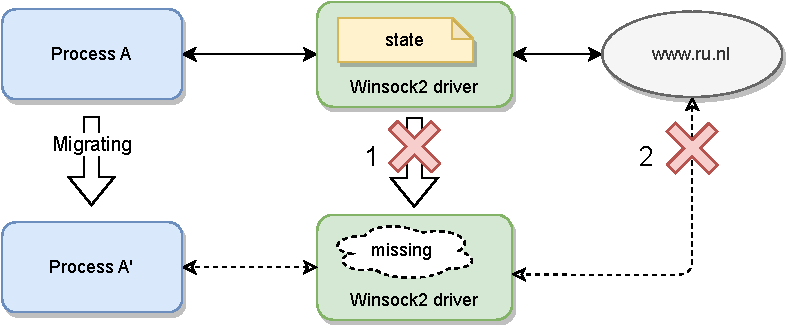
\includegraphics[width=\textwidth]{images/networking.drawio.pdf}
	
	\caption{1: The connection between Winsock2 driver and process is not restored. 2: Established connections are not restored.}
	\label{fig:networking}
\end{figure}

When the networking functionality can be restored, listening sockets can be restored as well.
Socket handles are file types with the name \texttt{/Device/Afd/}.
Sockets cannot be copied with \texttt{DuplicateHandle}, but \texttt{WSADuplicateSocketA} has to be used instead.\footnote{\url{https://learn.microsoft.com/en-us/windows/win32/winsock/socket-handles-2}}
With \texttt{GetExtendedTcpTable}\footnote{\url{https://learn.microsoft.com/en-us/windows/win32/api/iphlpapi/nf-iphlpapi-getextendedtcptable}} we then can retrieve information such as listening IP address and port. With \texttt{getaddrinfo}, \texttt{socket}, \texttt{bind}, and \texttt{listen} we can create a listening socket. 

\paragraph{Established network connections}
As shown in \autoref{fig:networking} depicted by a 2, a network connection provides communication between two parties and currently only one side is restored. This is the case with more handles (see \autoref{sec:other-end}). When malware is migrated while a TCP connection is active, the receiving server will not be able to process the restored connection. This may be a possible showstopper. Unless of course the malware is resilient to TCP connections dropping and then restarts them.

%\section{What are fundamental showstoppers?}
%\label{sec:showstoppers}

%\section{Reflection on (im)possibilities}

% === FUTURE WORK ===
\chapter{Future work}
\label{ch:future-work}

\section{Extension}
Because of time constraints and the complexity of process migration, our implementation is incomplete. To migrate a broader set of processes, we recommend the following extensions.

\paragraph{A more sound migration of memory} The migration of memory is already very sufficient. However, some improvements can be made for possibly a more stable destination process. Future research could look into the following: 
\begin{enumerate}
	\item Allocate file mappings with the file mapping API. 
	\item Also migrate the ASLR seed, to have future heap allocation and DLL loads equal on the source and destination process. 
	\item Perform process hollowing on the destination process first to create a more empty canvas to restore from. 
	\item Resolve the issue that the \texttt{USER\_SHARED\_DATA} and \texttt{HYPERVISOR\_SHARED\_DATA }are not migratble.
\end{enumerate}

\paragraph{Implement more handles}
As mentioned in \autoref{ch:handles}, we have not implemented every type of handle. We recommend future work to strive towards implementing a more complete set of handles, for example, the ALPC port mentioned in \autoref{sec:turian}. A kernel driver could be developed to retrieve more information about handles (see \autoref{sec:background-handles}). The types of handles we recommend implementing first are networking, registry keys, named pipes, and thread handles.

\paragraph{GUI applications}
Intuitively we expect that graphics add a lot of complexity to the migration. Since most malware does not have a graphical interface, we left GUI applications out of scope. With other applications in mind, this extension may be required.
%\todo{Why is this hard?}

\paragraph{32-bit applications and other Windows versions}
Malware is also developed as a 32-bit application for compatibility reasons, since next to 32-bit machines, 64-bit machines are also able to run 32-bit processes. It is also aimed toward other Windows versions. Our current implementation is architecture and version dependent. Future work could extend our implementation to support more architectures and Windows versions. The PE header, thread context, PEB, and TEB will be different compared to 64-bit. We expect porting to 32-bit processes would take 2 to 3 weeks. We expect porting to Windows 11 would take one week.

%\paragraph{More formal verification} ...

\section{Different applications}
In this thesis, we aimed towards using process migration for malware analysis. As shown in \autoref{ch:related-work}, process migration has uses in different applications. The list below describes possible different applications for process migration.

\paragraph{Use process migration for fuzzing}
Since we checkpoint a process we can use our implementation as a forking server to fuzz on a cluster of machines, as discussed in \autoref{sec:process-migration}. Process migration may be useful when one aims to use a computer cluster for fuzzing.

\paragraph{For rollback recovery}
Since we have created a checkpointing method for running processes, this may also be used to recover processes from crashes in Windows. By checkpointing at intervals and recording I/O, we can roll back to the previous checkpoint when a crash has occurred and replay the I/O traffic. More information about rollback recovery can be found online~\cite{chung1999winckp}.

% ------------------------------------

\chapter{Conclusion}
\label{ch:conclusion}

% Wat is gelukt zoals we hadden voorzien
% Was is verassend?
% Wat lukt absoluut niet?
% Wat kan je daar nog aan doen?
% Vooruit blik, aanbevelingen

In this thesis, we worked towards migrating a running Windows 10 process from one machine to another.
At the start of our research, we and others were skeptical about whether process migration would be possible on Windows. Now, we have demonstrated its feasibility by providing a proof of concept. We achieved this by checkpointing the state of a process and restoring a process from this state on the destination machine. Threads, memory, and some common external resources, such as files and semaphores, can be migrated by our implementation.
\looseness=-1

We divided the problem of process migration into smaller problems, starting with the simplest toy program we could imagine and gradually increasing the complexity. This approach served us well, as we were able to reach the first milestones early on in the research, confirming process migration was indeed possible.
\looseness=-1

We started this thesis with little knowledge about process migration and Windows internals. We spent around two months developing an understanding of Windows and related work. The official documentation from Microsoft for the Windows API~\cite{win32-api} was very useful as most system calls are well documented. Furthermore, the book ``Windows Internals''~\cite{windows-internals}\cite{windows-internals-2} was crucial for understanding the core components in Windows 10.

In \autoref{ch:related-work}, we describe tools for checkpointing in the literature. Most of them were developed for Linux~\cite{ansel2009dmtcp}\cite{paul2006BLCR}\cite{criu} and those developed for Windows~\cite{chung1999winckp} are outdated and not publicly available anymore.

We began our implementation by migrating a toy program consisting of two assembly instructions in \autoref{ch:shellcode}. We migrated the thread context and the memory page containing the toy program. Implementing this took less than two weeks. We learned that a small error already results in a crash.
We expanded this by migrating all the virtual memory of a process in \autoref{ch:memory}, such as the stack, heap, program image, and loaded DLLs. By performing better process initialization (see \autoref{sec:memory-main}) and adjusting the field in the PEB (see \autoref{sec:PEB}), we were able to restore the heap and stack. Most issues with migrating memory were solved, in around seven weeks. 

In \autoref{ch:handles}, we describe how to migrate resources outside the process, namely file handles, console handles, events, mutexes, and semaphores.
Handles have been more difficult to implement than expected. Our solution in its current state, supports just the most common handle types.
In \autoref{ch:real-world} we attempted to migrate a real-world malware sample of \textit{Turian} and demonstrate what still goes wrong.
As a result, we conclude that further research is needed to figure out how to query every type of handle and especially to support migrating the networking capabilities. 

Still, process migration is undoubtedly possible and we conclude our implementation is a start for the transfer of real-world malware.
We expect that by adding support for a wider variety of handles, it will become possible to migrate even more complex processes.

% - Wat je nu ook al kan doen: zet in je conclusie hoofstuk kun alvast
%   een opmerking zetten om je eraan te herinneren dat je tzt hier een
%   zin antwoord gaat geven op de vraag of a) vs b) haalbaar bleek.  De
%   tekst hiervoor kun je nu al grotendeels schijven:

%   "Bij de start vh onderzoek was het nog niet duidelijk of a)
%    vs b) (as defined in Section x.y) haalbaar was, maar uiteindelijk
%    bleek ?? niet haalbaar (as discussed in Section z.w) maar
%    ?? wel, as demonstrated by our solution in Chapter U."

%   Dit soort reminders zijn handig, want over een paar weken kies je
%   mogelijk voor a) vs b) en over een paar maanden ben je dan vergeten
%   dat er een uberhaupt een keuze was.

%   Het aantal terugverwijzingen is de voorbeeldzin hierboven is wat
%   overdreven, maar kan het nooit kwaad om er in eerste instantie veel
%   van dit soort verwijzingen in tekst zetten, omdat je dan gedwongen
%   wordt om even sanity check te doen op de consistentie & volledigheid
%   van de hele tekst vd scriptie.

\appendix
\chapter{Checkpoint file format}
\label{ap:fileformat}

\begin{tabular}{p{0.22\textwidth-2\tabcolsep} p{0.22\textwidth-2\tabcolsep} p{0.56\textwidth-2\tabcolsep} }
	\hline
	\textbf{Type} & \textbf{Name} & \textbf{Description } \\
	\hline
%	PROCESSENTRY32 & processEntry \\
%	PRTL\_USER\_PROCESS\_PARAMETERS & ProcessParameters \\
	\texttt{*VOID} & PebBaseAddress & Address of PEB \\
	\texttt{PEB} & PEB & Process Environment Block \\
	\texttt{TEB} & TEB & Thread Environment Block\\
	\texttt{[]CONTEXT} & threads & Thread context of all threads \\
	\texttt{[]Memory} & memory & List of all memory pages \\
	\texttt{[]Object} & objects & List of all handle objects \\
	\hline
\end{tabular}

\section{Definition of \texttt{Memory}}
\begin{tabular}{p{0.22\textwidth-2\tabcolsep} p{0.22\textwidth-2\tabcolsep} p{0.56\textwidth-2\tabcolsep} }
	\hline
	\textbf{Type} & \textbf{Name} & \textbf{Description } \\
	\hline
	\texttt{MEMORY\_BASIC\_INFORMATION} & & Details about the memory page \\
	\texttt{[]BYTE} & buffer & contents of memory page \\
	\hline
\end{tabular}

\section{Definition of \texttt{Object}}
\begin{tabular}{p{0.22\textwidth-2\tabcolsep} p{0.22\textwidth-2\tabcolsep} p{0.56\textwidth-2\tabcolsep} }
	\hline
	\textbf{Type} & \textbf{Name} & \textbf{Description } \\
	\hline
	\texttt{ULONG} & address & Address of handle \\
	\texttt{String} & type & type of handle \\
	\texttt{String} & name & name of handle \\
	\texttt{DWORD} & ftype & file type \\
	\texttt{LARGE\_INTEGER} & fpos & position in file \\
	\texttt{[]BYTE} & buffer & contents of file \\
	\hline
\end{tabular}

\printbibliography[heading=bibintoc]
%\printbibliography[heading=bibintoc,nottype=software]
%\printbibliography[type=software,title={List of Software}]


%\newgeometry{textwidth=1.2\textwidth,top=6em,
%            bottom=6em}
%\chapter{Code of checkpointing process}
%\pagestyle{empty}
%\pagenumbering{gobble}
%\lstset{numbers=none}
%%\lstset{basicstyle=\ttfamily\scriptsize}
%\lstset{basicstyle=\ttfamily\tiny}
%\lstinputlisting[label=lst:copy-code,language={[Visual]C++},caption={}]{code.cpp}
%\restoregeometry

\end{document}
